\chapter{Законы сохранения для различных динамических характеристик атмосферы}
Для изучения атмосферных процессов часто удобнее использовать уравнения сохранения не для исходных переменных (компонентов скорости), а для некоторых характеристик, причем таких, которые сохранялись бы в движущейся частице. Такие новые переменные называются инвариантами, т.к. они в движущейся частице сохраняются. Термодинамические адиабатические инварианты -- энтропия, потенциальная температура, псевдо-потенциальная температура получили широкое распространение в 20-е -- 30-е годы прошлого столетия. Адиабатические инварианты динамического характера начали изучаться позднее. Сюда относятся в прежде всего понятия вихря и потенциального вихря. Первый из них является инвариантом лишь в случае плоского течения и несжимаемой жидкости, второй является инвариантом даже в условиях сжимаемой атмосферы. В анализе используются также уравнения сохранения энергии и ряд других уравнений. Выводам этих уравнений и будет посвящена настоящая глава. Все они достаточно широко используются для диагностики моделируемых течений и лучшего понимания механизма образования различных атмосферных циркуляций. 

Вывод соответствующих уравнений будет сделан в декартовой системе координат. В отдельных случаях будут даны их выражения в других системах, но уже без подробного вывода. Поскольку вязкие члены всегда действуют одинаково: способствуют затуханию циркуляции или энергии, мы будем рассматривать для простоты случай идеальной жидкости и иметь дело со следующей системой:

    \begin{align}
        \fd{u} = -\alpha\pd{p}{x}+fv  \label{eq:ch10-DuDt} \\
        \fd{v} = -\alpha\pd{p}{y}-fu \label{eq:ch10-DvDt}  \\
        \fd{w} = -\alpha\pd{p}{z}-g \label{eq:ch10-DzDt}  
    \end{align}
Здесь $\alpha=\frac{1}{\rho}$ -- удельный объем жидкости (газа). Он в данном случае удобнее, чем плотность, т.к. дает более простые выражения при применении операторов дифференцирования. 

\section{{\color{done}Уравнение завихренности}} \label{ch10.1}
Наблюдая за каким-либо объектом в движущийся жидкости или газе мы часто можем заметить, что в движении присутствует вращательный компонент. Если бросить палку в речку, то можно заметить, что она не просто переносится потоком, а совершает одновременно вращательные движение. Это значит, что жидкие частицы, действующие на палку, имеют вращательный компонент. В атмосфере мы непосредственно наблюдаем вращение в мелких вихрях, если частицы воздуха вовлекают в свою циркуляцию какие-нибудь легкие частицы: листья или снежинки. В более крупном масштабе мы можем наблюдать вращательные движения по полю облачности или радиолокационного эха в атмосферных вихрях различного масштаба: тропических и внетропических циклонах. 

В атмосфере вращение частиц происходит частично вследствие термодинамического возбуждения и частично под действием вращения Земли. При изучении динамики атмосферы бывает полезно понять, каким образом генерируется вихревой компонент в движении частицы. При изучении кинематики жидкости было показано, что вектор скорости может быть представлен в виде ряда компонентов: дивергентного, вихревого, трансляционного и деформационного. Ротационный компонент скорости играет в этом ансамбле заметную роль. Идея вывода уравнения вихря состоит в том, чтобы понять, под действием каких процессов может увеличиваться (или убывать) завихренность в движущийся частице или в фиксированной точке пространства и сделать вывод о том, например, усилится циклоническая или антициклоническая циркуляция. Наиболее часть в задачах метеорологии оперируют с вертикальной составляющей завихренности, однако для более полного понимания процесса, лучше рассмотреть компоненты завихренности по всем координатам. Это связано с тем, что горизонтальная завихренность может переходить в вертикальную и наоборот. Кроме того, получив покомпонентные уравнения для завихренности легче понять векторную форму ее записи. Для атмосферы мы можем написать уравнения для относительной и абсолютной завихренности. Начнем с вывода уравнений относительной завихренности.

\begin{warn}
    Абзац ниже нужно слинковать с 1 и 2 главой, где будет говориться о завихренности в базовом (дифференциальном) смысле.
\end{warn}

Как отмечалось в главах \ref{ch1} и \ref{ch2} ({\color{red} ссылки на уравнения завихренности в их базовой форме}) завихренность вдоль осей $Ox$, $Oy$ и $Oz$ имеет следующий вид:
\begin{equation}
    \omega_x = \pd{w}{y}-\pd{v}{z}; \:\: \omega_y = \pd{u}{z}-\pd{w}{x}; \:\:\omega_z = \pd{v}{x}-\pd{u}{y}.
\end{equation}

Начнем последовательно вывод уравнений компонентов завихренности по всем осям. Для получения эволюционного уравнения для компонента $\omega_x$ нужно в левой части результирующего уравнения иметь слагаемое $\td{\omega_x}{t}$. Применим к уравнению (\ref{eq:ch10-DvDt}) оператор $-\pd{}{z}$, а к уравнению $\ref{eq:ch10-DzDt}$ оператор $\pd{}{y}$, будем иметь
\begin{align*}
    -&\pd{}{t}\pd{v}{z}-\pd{u}{z}\pd{v}{x}-u\pd{}{x}\pd{v}{z}-\pd{v}{z}\pd{v}{y} - 
    v\pd{}{y}\pd{v}{z}-\pd{w}{z}\pd{v}{z}-w\pd{}{z}\pd{v}{z} = 
    \pd{\alpha}{z}\pd{p}{y}+\alpha\frac{\partial^2p}{\partial y \partial z} + f\pd{u}{z} \\
    &\pd{}{t}\pd{w}{y}+\pd{u}{y}\pd{w}{x}+u\pd{}{x}\pd{w}{y}+\pd{v}{y}\pd{w}{y} +
    v\pd{}{y}\pd{w}{y}+\pd{w}{y}\pd{w}{z}+w\pd{}{z}\pd{w}{y} = 
    -\pd{\alpha}{y}\pd{p}{z}-\alpha\frac{\partial^2p}{\partial y \partial z} 
\end{align*}
Складывая и группируя члены этих уравнений, получаем
\begin{warn}
    исправить наблу (+u):
\end{warn}

\begin{equation*}
    \td{\omega_x}{t}+\omega_x(\nabla_{yz})-\pd{u}{z}\pd{v}{x}+\pd{u}{y}\pd{w}{x} = \left( \pd{\alpha}{z}\pd{p}{y} - \pd{\alpha}{y}\pd{p}{z} \right) + f\pd{u}{z},
\end{equation*}
здесь $\nabla_{yz} = \pd{v}{y} +\pd{w}{z}$ -- дивергенция в плоскости $yx$. 
Добавляя и вычитая в левой части $\pd{u}{z}\pd{u}{y}$, получим
\begin{equation*}
    -\pd{u}{z}\pd{v}{x}+\pd{u}{y}\pd{w}{x}+\pd{u}{z}\pd{u}{y}-\pd{u}{z}\pd{u}{y} = -\pd{u}{z} \left( \pd{v}{x}-\pd{u}{y} \right) - \pd{u}{y} \left( \pd{u}{z} - \pd{w}{x} \right).
\end{equation*}
Перенося часть членов из левой част ив правую, получаем
\begin{equation*}
    \td{\omega_x}{t} = -\omega_x(\nabla_{yz}) + \omega_z\pd{u}{z}+\omega_y\pd{u}{y}+f\pd{u}{z}+ \left( \pd{\alpha}{z}\pd{p}{y} - \pd{\alpha}{y}\pd{p}{z} \right)
\end{equation*}
или, окончательно,
\begin{equation}
\label{eq:ch10_omegax}
    \td{\omega_x}{t}=
    \ub{\vphantom{\left( \pd{a}{z}\pd{p}{y} \right)}(\omega_z+f)\pd{u}{z} + \omega_y\pd{u}{y}}_{1}
    \ub{\vphantom{\left( \pd{a}{z}\pd{p}{y} \right)}-\omega_x\nabla_{yz}}_{2}+
    \ub{\left( \pd{\alpha}{z}\pd{p}{y} - \pd{\alpha}{y}\pd{p}{z} \right)}_{3}
\end{equation}

Для получения эволюционного уравнения $y$-компоненты завихренности $\omega_y$ применим к уравнению (\ref{eq:ch10-DuDt}) оператор $\pd{}{z}$, а к уравнению \ref{eq:ch10-DzDt} оператор $-\pd{}{x}$

\begin{multline*}
    \pd{}{t}\pd{u}{z}+
        \pd{u}{z}\pd{u}{x} + u\pd{}{x}\pd{u}{z} +
        \pd{v}{z}\pd{u}{y} + v\pd{}{y}\pd{u}{z} +
        \pd{w}{z}\pd{u}{z} + w\pd{}{z}\pd{u}{z} = \\
    = -\pd{\alpha}{z}\pd{p}{x}-\alpha\frac{\partial^2p}{\partial x \partial z} + 
    f\pd{v}{z} 
\end{multline*}
\begin{multline*}
    -\pd{}{t}\pd{w}{x}-
        \pd{u}{x}\pd{w}{y} - u\pd{}{y}\pd{w}{x} -
        \pd{v}{x}\pd{w}{y} - v\pd{}{y}\pd{w}{x} -
        \pd{w}{x}\pd{w}{z} - w\pd{}{z}\pd{w}{x} = \\
    = \pd{\alpha}{x}\pd{p}{z}+\alpha\frac{\partial^2p}{\partial x \partial z} 
\end{multline*}
% \begin{align*}
%     &\pd{}{t}\pd{u}{z}+
%         \pd{u}{z}\pd{u}{x} + u\pd{}{x}\pd{u}{z} +
%         \pd{v}{z}\pd{u}{y} + v\pd{}{y}\pd{u}{z} +
%         \pd{w}{z}\pd{u}{z} + w\pd{}{z}\pd{u}{z} = \\
%     &= -\pd{\alpha}{z}\pd{p}{x}-\alpha\frac{\partial^2p}{\partial x \partial z} + 
%     f\pd{v}{z} \\
%     &-\pd{}{t}\pd{w}{x}-
%         \pd{u}{x}\pd{w}{y} - u\pd{}{y}\pd{w}{x} -
%         \pd{v}{x}\pd{w}{y} - v\pd{}{y}\pd{w}{x} -
%         \pd{w}{x}\pd{w}{z} - w\pd{}{z}\pd{w}{x} = \\
%     &= \pd{\alpha}{x}\pd{p}{z}+\alpha\frac{\partial^2p}{\partial x \partial z} 
% \end{align*}
Складывая эти уравнения и группируя члены, получаем
\begin{equation*}
    \td{\omega_y}{t}+\omega_y(\nabla_{xz})+\pd{v}{z}\pd{u}{y}-\pd{v}{x}\pd{w}{y} = \left( \pd{\alpha}{x}\pd{p}{z} - \pd{\alpha}{z}\pd{p}{x} \right) + f\pd{v}{z},
\end{equation*}
здесь $\nabla_{xz} = \pd{u}{x} +\pd{w}{z}$ -- дивергенция в плоскости $xz$. 
Добавляя и вычитая в левой части этого уравнения $\pd{v}{z}\pd{v}{x}$, будем иметь
\begin{equation*}
    -\pd{v}{z}\pd{u}{y}-\pd{v}{x}\pd{w}{y}+\pd{v}{z}\pd{v}{x}-\pd{v}{z}\pd{v}{x} = -\pd{v}{z} \omega_z - \pd{v}{x} \omega_x.
\end{equation*}
Группируя дополнительно члены и перенося часть их них в правую часть уравнения, получим окончательно
\begin{equation}
\label{eq:ch10_omegay}
    \td{\omega_y}{t}=
    \ub{\vphantom{\left( \pd{\alpha}{z}\pd{p}{y} \right)}(\omega_z+f)\pd{v}{z} + \omega_x\pd{v}{x}}_{1}
    \ub{\vphantom{\left( \pd{\alpha}{z}\pd{p}{y} \right)}-\omega_y\nabla_{xz}}_{2}+
    \ub{\left( \pd{\alpha}{x}\pd{p}{z} - \pd{\alpha}{z}\pd{p}{x} \right)}_{3}.
\end{equation}

Для получения эволюционного уравнения для вертикальной компоненты завихренности $\omega_z = \pd{u}{x}=\pd{v}{y}$ применим к уравнению (\ref{eq:ch10-DuDt}) оператор $-\pd{}{y}$, а к уравнению (\ref{eq:ch10-DvDt}) оператор $\pd{}{x}$ 
\begin{align*}
    -\pd{}{t}\pd{u}{y}-
        \pd{u}{y}\pd{u}{x} - u\pd{}{x}\pd{u}{y} -
        \pd{v}{y}\pd{u}{y} - v\pd{}{y}\pd{u}{y} -
        \pd{w}{y}\pd{u}{z} - w\pd{}{z}\pd{u}{y} = \\
    \pd{\alpha}{y}\pd{p}{x} + 
    \alpha\frac{\partial^2p}{\partial x \partial y} - \pd{f}{y}v - f\pd{v}{y} \\
    \pd{}{t}\pd{v}{x}+
        \pd{u}{x}\pd{v}{x} + u\pd{}{x}\pd{v}{x} +
        \pd{v}{x}\pd{v}{y} + v\pd{}{y}\pd{v}{x} +
        \pd{w}{x}\pd{v}{z} + w\pd{}{z}\pd{v}{x} = \\
    -\pd{\alpha}{x}\pd{p}{y} - 
        \alpha\frac{\partial^2p}{\partial x \partial y} - 
        \cancelto{0}{\pd{f}{x}}u - f\pd{u}{x} 
\end{align*}
Складывая эти уравнения и группируя члены, получаем
\begin{equation*}
    \td{\omega_z}{t}+\omega_z(\nabla_{xy})-\pd{w}{y}\pd{u}{z}+\pd{w}{x}\pd{v}{y} = \left( \pd{\alpha}{y}\pd{p}{x} - \pd{\alpha}{x}\pd{p}{y} \right) - f\nabla_{xy} - \beta v,
\end{equation*}
здесь $\nabla_{xy}=\pd{u}{x}+\pd{v}{y}$ -- дивергенция в плоскости $xy$. Добавляя и вычитая $\left( \pd{w}{x}\pd{w}{y} \right)$, будем иметь
\begin{equation*}
    -\pd{w}{y}\pd{u}{z}+\pd{w}{x}\pd{v}{y}+\pd{w}{x}\pd{w}{y}-\pd{w}{x}\pd{w}{y} = 
    -\pd{w}{x} \ub{ \left( \pd{w}{y} - \pd{v}{z} \right) }_{\omega_x} 
    -\pd{w}{y} \ub{ \left( \pd{u}{z} - \pd{w}{x} \right) }_{\omega_y} 
\end{equation*}
Группируя дополнительно члены и перенося часть их них в правую часть уравнения, получим окончательно
\begin{equation}
\label{eq:ch10_omegaz}
    \td{\omega_z}{t}=
    \ub{\vphantom{\left( \pd{\alpha}{z}\pd{p}{y} \right)}\omega_x\pd{w}{x} + \omega_y\pd{w}{y} -\beta v }_{1} - 
    \ub{\vphantom{\left( \pd{\alpha}{z}\pd{p}{y} \right)}
    \left( \omega_z + f \right) \nabla_{xy}}_{2}+
    \ub{\left( \pd{\alpha}{y}\pd{p}{x} - \pd{\alpha}{x}\pd{p}{y} \right)}_{3}.
\end{equation}
Из этого и аналогичных уравнений для $\omega_x$ и $\omega_y$ видно, что индивидуальная скорость изменения относительной завихренности зависит от трех групп членов, каждую их которых можно рассматривать как завихренность вокруг соответствующей оси. Рассмотрим конкретно вертикальный компонент завихренности, а к сравнению разных компонент завихренности придем позже. 

Первую группу слагаемых (три первых слагаемых в правой части уравнения \ref{eq:ch10_omegaz}) называют по-разному: эффектом вихревой трубки, членом наклона завихренности (tilting) или членом закручивания (twisting). Эти члены характеризуют превращение завихренности по двум другим осям в завихренность вдоль данной оси. В случае $\omega_z$ происходит переход двух горизонтальных компонент в вертикальную, т.е. горизонтальные вихревые трубки как бы наклоняются, именно поэтому поэтому члены и называются членами наклона. 
    \begin{figure}[h]
    \centering
    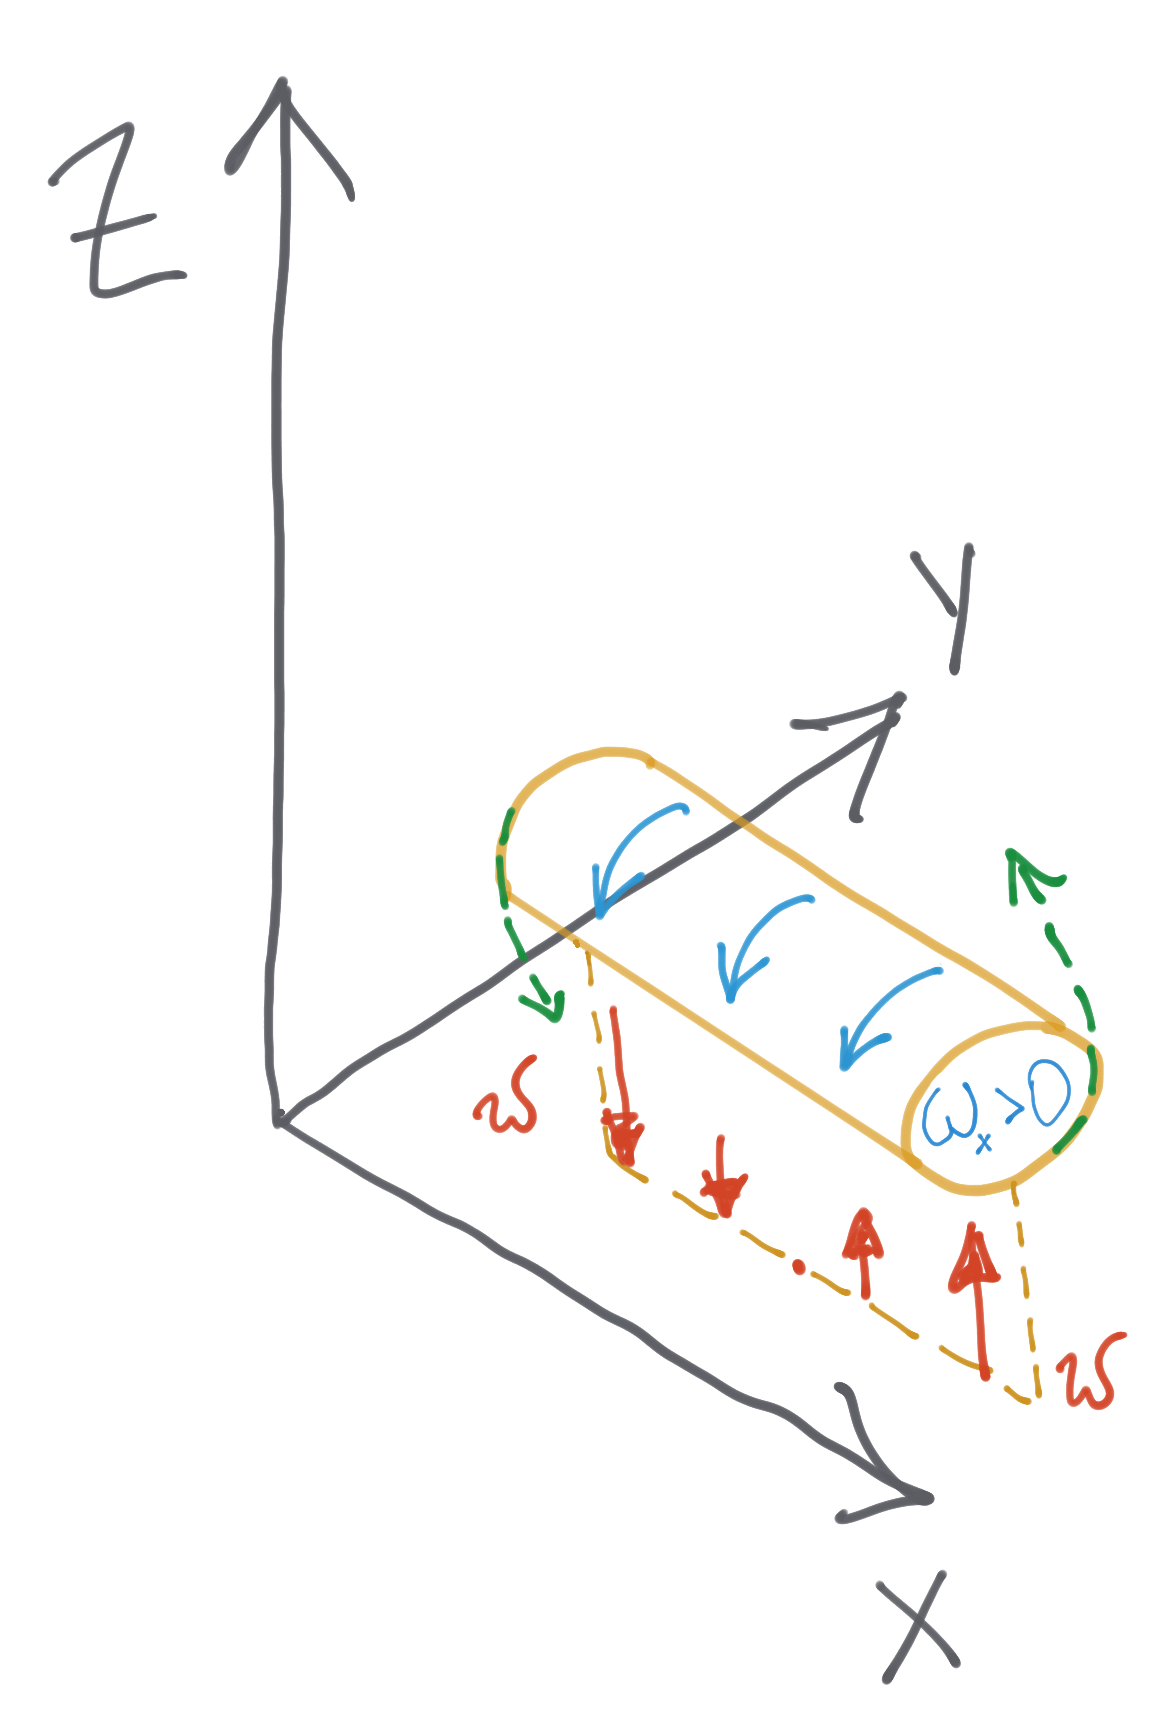
\includegraphics[width=0.5\linewidth]{pics/ch10.1.png}
    \caption{\label{fig:ch10.1}
    Пояснение условия члена наклона на примере действия члена $\omega_x\pd{w}{x}$
    }
    \end{figure}    
Поясним действие члена наклона на примере действия члена $\omega_x\pd{w}{x}$. Пусть для определенности $\omega_x > 0$, то есть вращение происходит против часовой стрелки и пусть распределение вертикальной скорости таково, что $\pd{w}{x}>0$ (красные стрелки на рисунке \ref{fig:ch10.1}). Тогда материальная кривая, образующая цилиндр и находящаяся первоначально в вертикальной плоскости $zOy$ и вдоль которой циркулирует воздух вокруг оси $Ox$, будет наклоняться вертикальными движениями так, как это показано пунктирными зелеными стрелками, и приведет к тому, что будет увеличиваться завихренность в вертикальном направлении $\left( \td{\omega_z}{t}>0 \right)$. Этот эффект существенен, так как позволяет переводить довольно большие значения $\omega_x$ и $\omega_y$ в $\omega_z$. 
\begin{warn}
    В рукописях (дополнение к стр 4) есть еще аналог масштабного анализа для одного частного случай. Я не уверен, что это нужно сюда вставлять.
\end{warn}
Если рассматриваются движения большого масштаба, то генерация завихренности может происходить также под действием $\beta$-эффекта. Необходимо отметить, что эта группа членов является источником и стоком завихренности.

Вторая группа членов (четвертое слагаемое в уравнении (\ref{eq:ch10_omegaz})) характеризует влияние дивергенции в плоскости, нормальной к компоненту завихренности, на усиление или ослабление завихренности. Эти члены оказывают воздействие только в том случае, когда завихренность уже существует. 

Так как $\nabla_{xy}<0$ характеризует конвергенцию, то в этом случае уже существующая положительная завихренность усиливается (вихревая трубка сужается и циркуляция в ней становится сильнее), а в случае дивергенции -- ослабевает (вихревая трубка расширяется). Этот член часто называют членом вытягивания (stretching), поскольку он вытягивает вихревую трубку. 
    \begin{figure}[h]
    \centering
    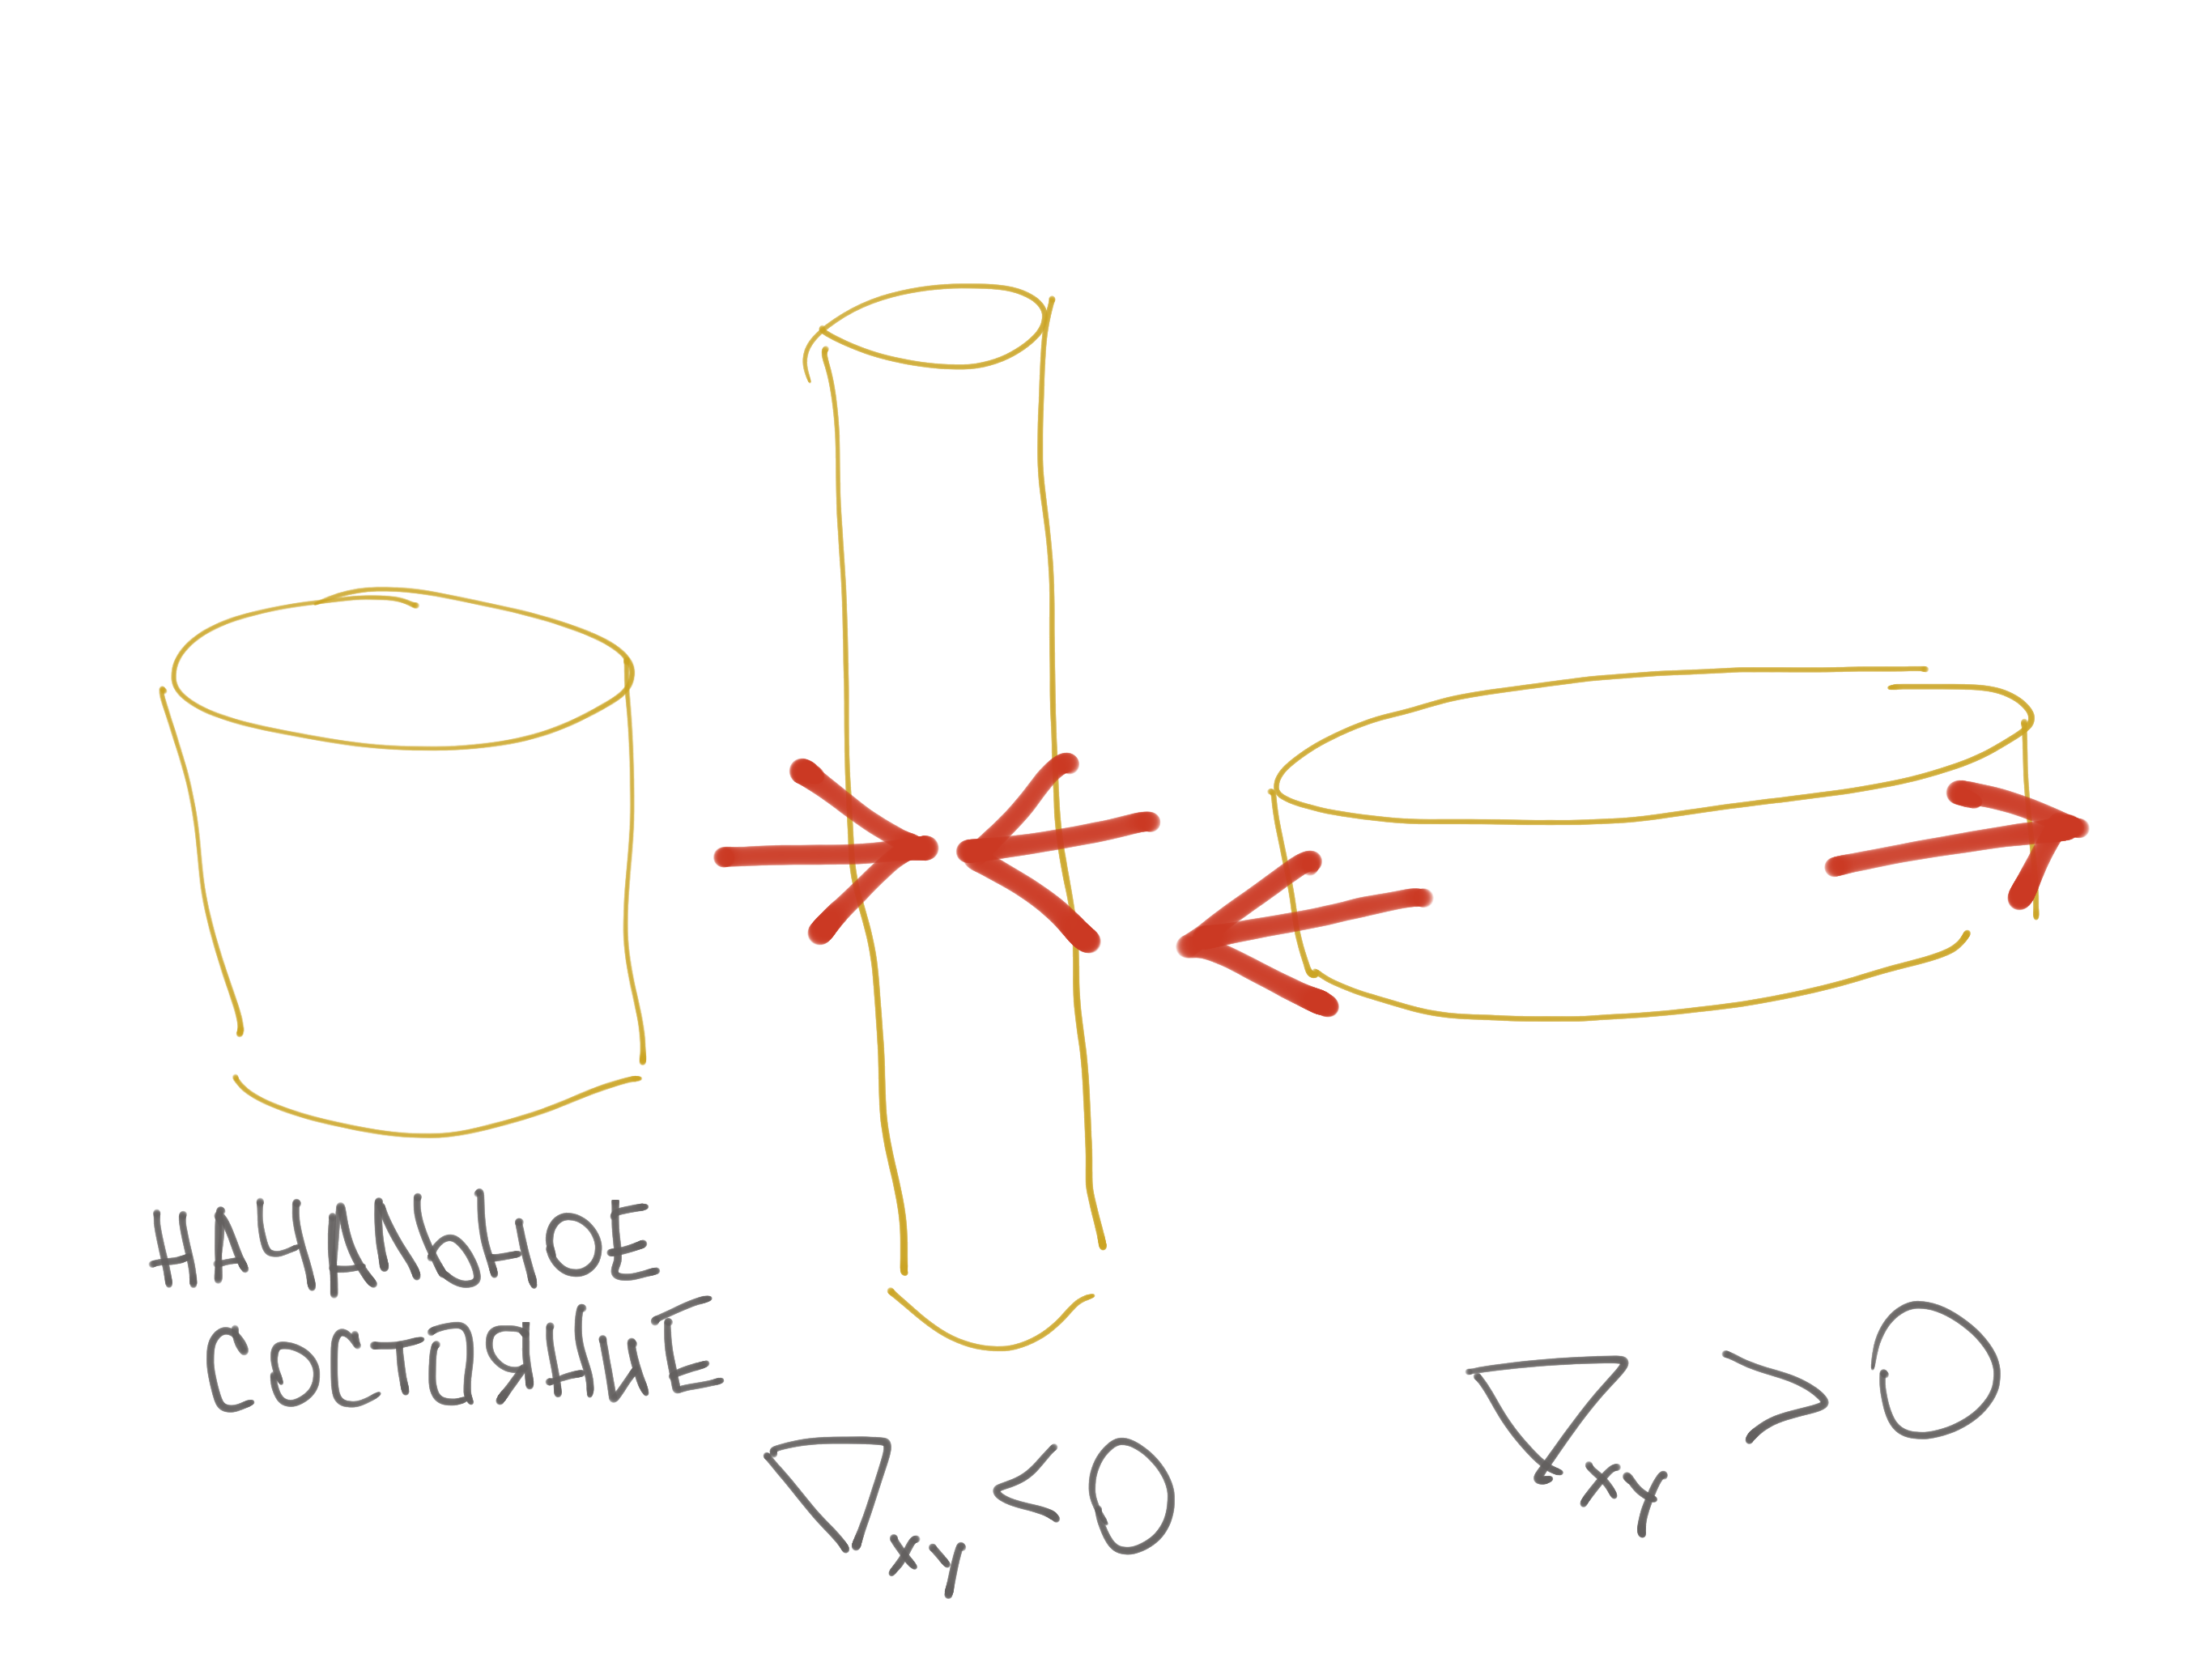
\includegraphics[width=0.5\linewidth]{pics/ch10.2.png}
    \caption{\label{fig:ch10.2}
    Пояснение условия члена вытягивания
    }
    \end{figure}    
Вертикальное вытягивание колонки воздуха увеличивает его завихренность. Процесс здесь подобен тому, который можно наблюдать у фигуристов. Сначала они раскручиваются с расставленными руками, а затем прижимают их к телу много усиливая скорость вращения. При необходимости замедлить вращение руки снова открываются. Прижимание и открытие рук подобно действию конвергенции и дивергенции, соответственно. 

Последних два слагаемых в уравнении (\ref{eq:ch10_omegaz}) описывают завихренность за счет бароклинности. Представим их в векторной форме:
\begin{equation*}
    \pd{\alpha}{y}\pd{p}{x}-\pd{\alpha}{x}\pd{p}{y}=\vec{k} \left( \nabla_hp \times \nabla_h\alpha \right) = \vec{k} \left( \nabla_hp \times \nabla_hT \right) \frac{R}{\rho}  
\end{equation*}
{\color{red}Вывод этой формулы будет сделан несколько позднее.} Графически действие этого члена представлено так: 
    \begin{figure}[h]
    \centering
    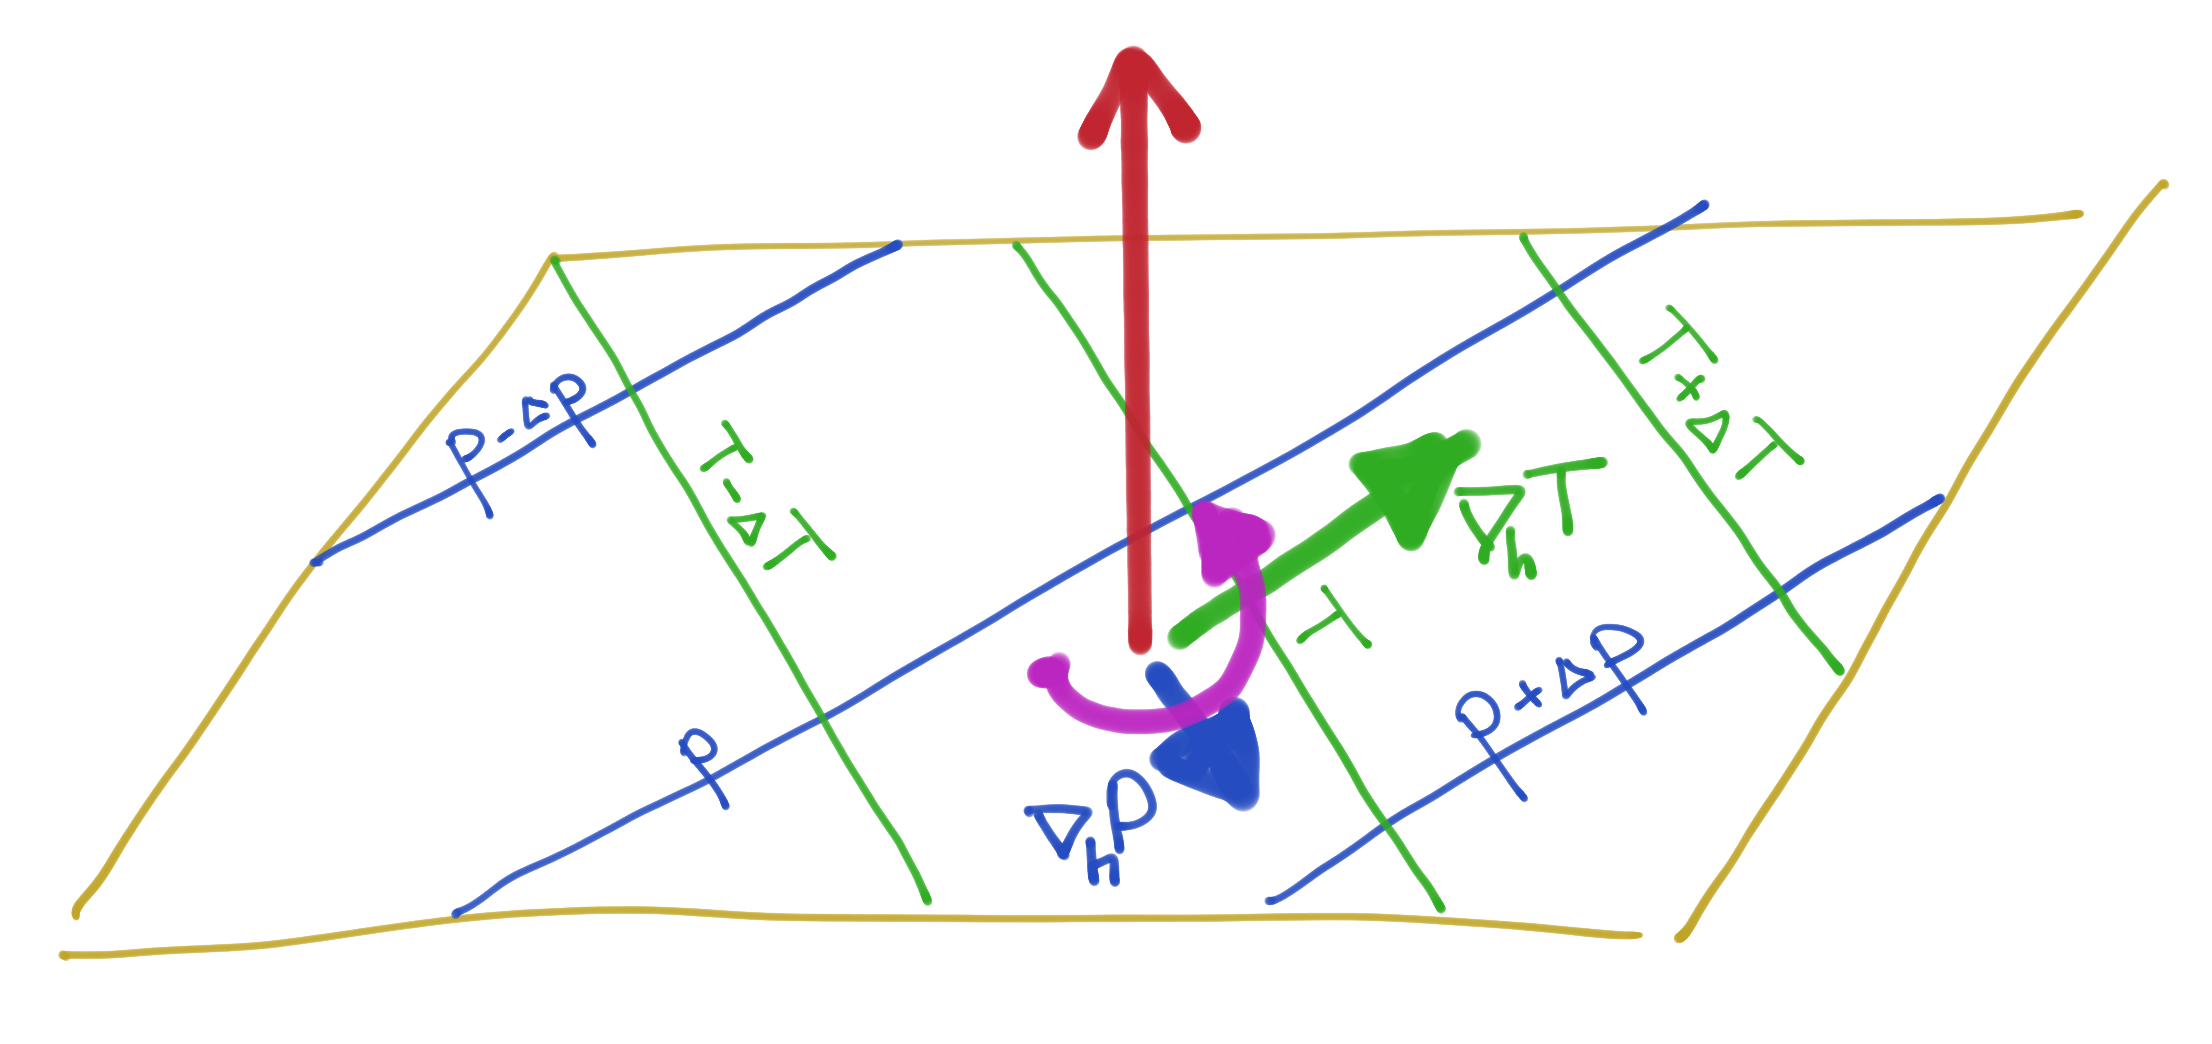
\includegraphics[width=0.9\linewidth]{pics/ch10.3.png}
    \caption{\label{fig:ch10.3}
    Пояснение действия члена бароклинности
    }
    \end{figure}    
Здесь $\nabla_h$ обозначает оператор горизонтального градиента. При направлении градиентов давления и температуры, изображенном на этом рисунке завихренность должна быть положительной и циркуляция происходить в направлении от конца вектора $\nabla_hp$ к концу вектора $\nabla_hT$ в направлении {\color{red}меньшего угла между ними} как это показано розовой стрелкой на рисунке \ref{fig:ch10.3}. 

Запишем теперь полученные нами уравнения для компонентов вихря более единообразно. Наши исходные компоненты завихренности имеют вид
\begin{align}
    \td{\omega_x}{t}&= (\omega_z+f)\pd{u}{z} + \omega_y\pd{u}{y}
    -\omega_x\nabla_{yz}+\left( \pd{\alpha}{z}\pd{p}{y} - \pd{\alpha}{y}\pd{p}{z} \right) \label{eq:ch10_omegax1} \\
    \td{\omega_y}{t}&=(\omega_z+f)\pd{v}{z} + \omega_x\pd{v}{x}
    -\omega_y\nabla_{xz}+\left( \pd{\alpha}{x}\pd{p}{z} - \pd{\alpha}{z}\pd{p}{x} \right) \label{eq:ch10_omegay1} \\
    \td{\omega_z}{t}&=
    \omega_x\pd{w}{x} + \omega_y\pd{w}{y} -\beta v - 
    \left( \omega_z + f \right) \nabla_{xy}+
    \left( \pd{\alpha}{y}\pd{p}{x} - \pd{\alpha}{x}\pd{p}{y} \right) \label{eq:ch10_omegaz1}.
\end{align}
Глядя на эти уравнения можно заметить, что имеется некоторая асимметрия в появлении силы Кориолиса в разных уравнениях. Это связано с тем, что не все компоненты ускорения силы Кориолиса были учтены в исходных уравнениях движения, а также с тем, что учитывалось только его изменение вдоль оси $y$. 

Чтобы сделать уравнения (\ref{eq:ch10_omegax1})-(\ref{eq:ch10_omegaz1}) более единообразными, прибавим и вычтем в каждом уравнении члены, которые превратят разные плоские дивергенции в полную дивергенцию в каждом уравнении. Добавляя и вычитая в правой части уравнения (\ref{eq:ch10_omegax1}) член $\omega_x\pd{u}{x}$, в уравнении (\ref{eq:ch10_omegay1}) $\omega_y\pd{v}{y}$, а в уравнении (\ref{eq:ch10_omegaz1}) $\omega_z\pd{w}{z}$, получим 
\begin{align}
    \td{\omega_x}{t}&= \omega_x\pd{u}{x} + \omega_y\pd{u}{y} + (\omega_z+f)\pd{u}{z} - \omega_x\nabla\vec{u}-\left( \pd{\alpha}{y}\pd{p}{z} - \pd{\alpha}{z}\pd{p}{y} \right) \label{eq:ch10_omegax2} \\
    \td{\omega_y}{t}&=\omega_y\pd{v}{y} + \omega_x\pd{v}{x} + (\omega_z+f)\pd{v}{z} -\omega_y\nabla\vec{u}-\left( \pd{\alpha}{z}\pd{p}{x} - \pd{\alpha}{z}\pd{p}{x} \right) \label{eq:ch10_omegay2} \\
    \td{\omega_z}{t}& = 
    \ub{\omega_x\pd{w}{x} + \omega_y\pd{w}{y} + \omega_z\pd{w}{z}}_{\romans{1}} 
    \ub{\vphantom{\omega_x\pd{w}{x} + \omega_y\pd{w}{y} + \omega_z\pd{w}{z}}-\beta v}_{\romans{2}} - 
    \ub{\vphantom{\omega_x\pd{w}{x} + \omega_y\pd{w}{y} + \omega_z\pd{w}{z}}\left( \omega_z + f \right) \nabla\vec{u}}_{\romans{3}}-
    \ub{\left( \pd{\alpha}{x}\pd{p}{y} - \pd{\alpha}{y}\pd{p}{x} \right)}_{\romans{4}} \label{eq:ch10_omegaz2}.
\end{align}

Посмотрим теперь, что представляют в этих уравнениях отдельные группы членов. В группе членов \romans{1} у нас присутствуют только вертикальная составляющая силы Кориолиса, т.к. проекции ускорения Кориолиса на оси $x=0$ и соответствующая производная от ускорения Кориолиса равны нулю. Поэтому мы можем добавить равные нулю компоненты ускорения Кориолиса в адвективные члены и написать их в векторной форме $\vec{\omega_a}\cdot\nabla\vec{U}$.  

Аналогично член \romans{2} $- \beta v$: по определению есть $\beta=\pd{f}{y}$. Если мы напишем полный оператор $\td{f}{t}=\fd{f}$, то т.к. $\pd{f}{x}=0$, $\pd{f}{z}=0$, $\td{f}{t}=v\pd{f}{y}=v\beta$. Поэтому мы можем вместо $-\beta v$ поставить в правой части $-\td{f}{t}$, перенести затем это в левую часть. Вспомним теперь, что горизонтальные компоненты силы Кориолиса были исключены, в противном случае там появились бы аналогичные (но равные нулю)  члены $\td{f_x}{t}$, $\td{f_y}{t}$. Если мы обозначим $\vec{\omega_a}=(\omega_x+f_x)\vec{i}+(\omega_y+f_y)\vec{j}+(\omega_z+f_z)\vec{k}$, то левая часть уравнений (\ref{eq:ch10_omegax2})-(\ref{eq:ch10_omegaz2}) в векторной форме будет $\td{\vec{\omega_a}}{t}$.

Аналогичным образом группа членов \romans{3} с дивергенцией может быть представлена в векторном виде как $\\vec{\omega_a}\nabla\vec{U}$. 

Группа бароклинных членов, у который был изменен знак на обратный в системе (\ref{eq:ch10_omegax2})-(\ref{eq:ch10_omegaz2}) по сравнению с системой (\ref{eq:ch10_omegax1})-(\ref{eq:ch10_omegaz1}) может также быть представлена в векторном виде. Вспомним, что $\vec{a}\times\vec{b}=(\vec{a}\times\vec{b})_x+(\vec{a}\times\vec{b})_y+(\vec{a}\times\vec{b})_z=\vec{i}(a_xb_z-a_zb_y)+\vec{j}(a_zb_x-a_xb_z)+\vec{k}(a_xb_y-a_yb_x)$. Сравнивая это выражение с группой членов \romans{4} в системе (\ref{eq:ch10_omegax2})-(\ref{eq:ch10_omegaz2}) увидим, что они представляют собой векторное произведение, только в качестве проекции вектора на соответствующую ось выступают соответствующие производные, т.е. сумма этих членов есть $\nabla\alpha\times\nabla P$. 

Таким образом система (\ref{eq:ch10_omegax2})-(\ref{eq:ch10_omegaz2}) может быть представлена в векторной форме следующим образом:
\begin{equation}
\label{eq:ch10-OmegaVec}
    \td{\omega_a}{t}=\vec{\omega_a}\cdot\nabla{\vec{U}} - \vec{\omega_a}\nabla\cdot\vec{U} - \nabla\alpha \times \nabla P
\end{equation}
Так как $d\alpha=d \left( \frac{1}{\rho} \right)=-\frac{1}{\rho^2}d\rho$, то уравнение ($\ref{eq:ch10-OmegaVec}$) может быть представлено также в виде
\begin{equation}
\label{eq:ch10-OmegaVec1}
    \td{\omega_a}{t}=\vec{\omega_a}\cdot\nabla{\vec{U}} - \vec{\omega_a}\nabla\cdot\vec{U} - \frac{1}{\rho^2} \left[ \nabla\rho \times \nabla P \right]
\end{equation}
С использование уравнения состояния его можно представить в виде
\begin{equation}
\label{eq:ch10-OmegaVec2}
    \td{\omega_a}{t}=\vec{\omega_a}\cdot\nabla{\vec{U}} - \vec{\omega_a}\nabla\cdot\vec{U} - \frac{1}{\rho T} \left[ \nabla T \times \nabla P \right]
\end{equation}
\begin{warn}
    Дать пояснение этому уравнению, стр 7а
\end{warn}
Если по какой-то причине удобнее записать векторное уравнение для относительного вихря, то оно имеет виду 
\begin{equation}
\label{eq:ch10-OmegaVec3}
    \td{\omega}{t}=\vec{\omega}\cdot\nabla{\vec{U}} - \vec{\omega}\nabla\cdot\vec{U} - 
    2\nabla(\vec{\Omega}\times\vec{U}) -\frac{1}{\rho T} \left[  \nabla T \times \nabla P \right]
\end{equation}

Часто бывает удобно использовать уравнение завихренности в изобарических координатах. Для простоты рассмотрим только уравнение для вертикального компонента завихренности. Не останавливаясь на выводе компонентов завихренности напишем их сразу. 
\begin{info}В порядке упражнения можете получить их самостоятельно, применяя правила дифференцирования сложной функции к оператору вихря в $z$-системе координат.\end{info}
Итак, в $p$-системе
\begin{equation}
    \omega_x = \pd{\tau}{y}-\pd{v}{z}; \:\: \omega_y = \pd{u}{z}-\pd{\tau}{x}; \:\:\omega_p = \pd{v}{x}-\pd{u}{y}.
\end{equation}
Для вывода уравнения для вертикального компонента нам достаточно первых двух уравнений движения.
\begin{align}
    -\pd{}{y} \bigg| \:\:\:\: \pd{u}{t}+\vec{V}\nabla_pu + \tau\pd{u}{p}&=-g\pd{H}{x}+fv \label{eq:ch10-dudt_p} \\
     \pd{}{x} \bigg| \:\:\:\: \pd{v}{t}+\vec{V}\nabla_pv + \tau\pd{v}{p}&=-g\pd{H}{y}-fu \label{eq:ch10-dudt_p},
\end{align}
где $\nabla_p=\pd{}{x}+\pd{}{y}$ -- плоский оператор дивергенции в $p$-системе. Применяя к (\ref{eq:ch10-dudt_p}) и (\ref{eq:ch10-dudt_p}) оператор вихря, получим
\begin{equation*}
    \td{ \left( \omega_p + f\right) }{t} = - \left( \omega_p+f \right)\nabla_p\vec{V}+\pd{\tau}{y}\pd{u}{p}-\pd{\tau}{x}\pd{v}{p}
\end{equation*}
Добавим и вычтем в правой части этого выражения $\pd{\tau}{x}\pd{\tau}{y}$, будем иметь
\begin{equation*}
    \pd{\tau}{y}\pd{u}{p} - \pd{\tau}{x}\pd{v}{p}+\pd{\tau}{x}\pd{\tau}{y}-\pd{\tau}{x}\pd{\tau}{y}.
\end{equation*}
Группируя члены, получаем
\begin{equation*}
    \pd{\tau}{y} 
    \ub{\left(  \pd{u}{p} - \pd{\tau}{x} \right)}_{\omega_y} + 
    \pd{\tau}{x} 
    \ub{\left( \pd{\tau}{y}-\pd{v}{p} \right)}_{\omega_x},
\end{equation*}
после чего окончательное уравнение вертикального компонента завихренности в изобарических координатах примет следующий вид: 
\begin{equation}
    \label{eq:ch10-DomegaDt_p}
    \td{}{t} \left( \omega_p + f \right) = -(\omega_p+f)\nabla_p\vec{V} + \omega_x\pd{\tau}{x}+\omega_y\pd{\tau}{y}.
\end{equation}
Основное отличие $\omega_p$ от $\omega_z$ состоит в том, что в нем отсутствует член, описывающий измерение завихренности в движущейся частице за счет изобаро- изостерических соленоидов (бароклинный член). Это происходит из-за того, что правые части уравнений движения в $p$-систем линейны (при перекрестном дифференцировании члены с геопотенциалом в правой части исчезают). В случае плоского течения $\tau=0$ и несжимаемой жидкости $\nabla_p\vec{V}=0$ вихрь становится динамическим инвариантом, т.е. имеет место равенство
\begin{equation}
    \td{}{t} \left( \omega_p + f \right) = 0
\end{equation}
Если движение рассматривается на $\beta$-плоскости, то этот динамический инвариант приобретает вид:
\begin{equation}
    \td{}{t}\omega_p=0
\end{equation}
В случае $z$-системы инвариантность абсолютной и относительной завихренности имеет место только при условии несжимаемой жидкости ($\rho=const$) и плоского течения ($w=0$).  Действительно в этом случае $\nabla\vec{U}=0$, бароклинный член также равен нулю из (\ref{eq:ch10-OmegaVec1}) имеем
\begin{equation}
    \td{\omega_a}{t}=0.
\end{equation}
Аналогично, при дополнительном постоянстве силы Кориолиса из (\ref{eq:ch10-OmegaVec3})
\begin{equation}
    \td{\omega}{t}=0.
\end{equation}
\begin{warn}
    В рукописях еще остались различные обрывки выводов и мыслей, если что...
\end{warn}


\section{{\color{done}Уравнение потенциального вихря}}
Определение потенциального вихря было дано в Эртелем в 1941 г. Им же и была доказана теорема о сохранении потенциального вихря. Эта теорема применима к расслоенной, термодинамической неоднородной атмосфере, в которой градиент энтропии не равен нулю $(\nabla S\neq0)$. Она гласит, что в такой среде при потенциальном характере внешних сил (гравитация), адиабатичности процессов и отсутствии диссипативных сил величина
\begin{equation}
    \label{eq:ch10-q}
    q=\left( \nabla S\cdot\nabla\times\vec{V} \right)/\rho
\end{equation}
обладает свойством сохранения в частице:
\begin{equation}
    \label{eq:ch10-dqdt}
    \td{q}{t}=0.
\end{equation}
Переменные $q$ в этих уравнениях называются потенциальным вихрем и представляет собой проекцию вихря на градиент энтропии (потенциальной температуры). 

\begin{info}
    Энтропия пропорциональна логарифму потенциальной температуры $S \sim \ln{\theta}$ (из курса физической метеорологии) 
\end{info}

Произведем вывод уравнения потенциального вихря. Исходными для нас будут уравнения движения без учета силы Кориолиса, уравнение сохранения массы и уравнение притока тепла. 
\begin{align}
    &\td{\vec{V}}{t} = -\frac{1}{\rho} \nabla P - \vec{k}g + \varepsilon F \label{eq:ch10-dudt_vec} \\
    &\td{\rho}{t}+\rho \nabla \Vec{V}=0 \label{eq:ch10-masscons} \\
    &\td{\sigma}{t} = \varepsilon Q \label{eq:ch10-temp}.
\end{align}
Здесь $\varepsilon$ -- некоторый коэффициент, при $\varepsilon=0$ жидкость идеальна, а происходящие в ней процессы адиабатичны. В уравнении притока тепла (\ref{eq:ch10-temp}) $\sigma=S/C_p$, где $S$ -- энтропия. Чтобы была понятна причина удобства использования $\sigma$, произведем переход от $S$ к $\sigma$. В главе \ref{ch03} было дано определение энтропии ({\color{red} ссылка на уравнение, когда оно будет готово}), которое воспроизведем снова.
\begin{warn}
    Этот текст надо надо перенести в Гл 3, а тут просто сослаться на него. 
\end{warn}
{\color{red}
В книге Леонтовича "Введение в гидродинамику и статистическая физика" дано следующее определение энтропии
\begin{equation}
    S = C_v \ln{T} + R \ln{v} + const, \label{eq:ch03-entropy}
\end{equation}
где $C_v$ -- удельная теплоемкость при постоянном объеме, $R$ -- газовая постоянная. Из уравнения состояния 
\begin{align}
    pv &= RT \:\:\:\: v=\frac{RT}{p} \label{eq:ch03-static1} \\
    p & =\rho R T \:\:\:\: T=\frac{p}{\rho R} \label{eq:ch03-static2}. \\
\end{align}
Исключим с помощью \ref{eq:ch03-static1} $v$ из \ref{eq:ch03-entropy}
    \[ S = C_v \ln{T} + R \ln{ \left[ \frac{RT}{p} \right]} = C_v \ln{T} + R \left[ \ln{R} + \ln{T} - \ln{p} \right]; \]
    \[ S = C_v \ln{T} +  \boxed{R \tikzmark{z1}\ln{R}}  + R \ln{T} - R \ln{p} +  co\tikzmark{z2}nst \]
        \begin{tikzpicture}[remember picture,overlay]
          \draw[->]
          ([shift={(2pt,-2pt)}]z1)
          -- ([shift={(2pt,-12pt)}]z1)
          -- node[midway, below] {$\scriptstyle const$} ([shift={(2pt,-12pt)}]z2)
          -- ([shift={(2pt,-2pt)}]z2);
        \end{tikzpicture}
    \[ S = ( C_v + R) \ln{T} - R \ln{p} + const,  \]
но $(C_v+R)=C_p$, поэтому
}
\begin{equation*}
    S = C_p \ln{T} - R \ln{p} + const.
\end{equation*}
Нам желательно заменить температуру $T$ плотностью, т.к. она входит в определение потенциального вихря. Сделаем это с помощью уравнения состояния 
    \[ S=C_p \ln{ \left[\frac{p}{\rho R} \right] } - R \ln{p} + const = C_p \left[ \ln{p} - \ln{\rho} - \ln{R} \right] - R \ln{p} + const, \]
    \[ S = \ub{(C_p - R)}_{C_p} \ln{p} - \boxed{C_p \tikzmark{z3} \ln{R} } - C_p \ln{R} + co\tikzmark{z4}nst
    \]
            \begin{tikzpicture}[remember picture,overlay]
          \draw[->]
          ([shift={(2pt,-6pt)}]z3)
          -- ([shift={(2pt,-12pt)}]z3)
          -- node[midway, below] {$\scriptstyle const$} ([shift={(2pt,-12pt)}]z4)
          -- ([shift={(2pt,-2pt)}]z4);
        \end{tikzpicture}
Группируя члены и учитывая, что $R=const$, получим
\[
S = C_v \ln{p} - C_p \ln{\rho} + const
\]
Разделив все члены на $C_p$, будем иметь
\begin{equation*}
    \sigma = \frac{S}{C_p} = \frac{C_v}{C_p} \ln{p} - \ln{\rho} + const = \frac{1}{\varkappa} ,
\end{equation*}
где $\varkappa=\frac{C_p}{C_v}$.

Это выражение удобно для нас тем, что в правой части уравнения вихря содержится член, куда входят плотность и давление (член с градиентом давления).

Итак, в новой переменной $\sigma$ определение потенциального вихря есть 
\[
q = ( \nabla \sigma \cdot \Vec{\Omega} ) / \rho, 
\]
где $\vec{\Omega}=\nabla \times \vec{V}$. Нам нужно показать, чему равно $\td{q}{t}$ в более общем случае и в адиабатическом в частности. Исходными уравнениями для этой цели будут уравнение относительного вихря (Фридмана), выведенное в разделе \ref{ch10.1} и уравнение притока тепла
\begin{align}
    &\td{ \vec{ \Omega} }{t} - (\vec{\Omega}\nabla)\vec{V} + \Omega \nabla\cdot\vec{V} = \frac{1}{\rho} \left( \nabla \rho \times \nabla p \right) + \varepsilon \nabla \times F \label{eq:ch10_relvort} \\
    &\td{\sigma}{t} = \varepsilon Q \label{eq:ch10_DsigmaDt}
\end{align}
Применим теперь оператор дифференцирования в направлении вектора $\vec{\Omega}$ к полной производной $\td{\sigma}{t}$
\begin{equation}
\label{eq:ch10-theta1}
    \rb{ \vec{\Omega}\nabla } 
    \rb{ \pd{}{t}+(\vec{V}\nabla) } \sigma.
\end{equation}
Применяя этот оператор нам нужно помнить, что желательно сгруппировать члены так, чтобы получить составляющие индивидуальной производной для $q\sim\vec{\Omega\nabla\sigma}$, т.е. члены
\begin{equation*}
    \pd{}{t} \ub{\rb{ \vec\Omega\nabla\sigma }}_{\sim q} + \vec{V}\nabla \ub{\rb{\vec{\Omega}\nabla\sigma}}_{\sim q}
\end{equation*}
Применяя этот оператор к 1-ому слагаемому в (\ref{eq:ch10-theta1}) получим $ \vec{\Omega}\pd{}{t} \rb{\sigma}$, но нам нужно вынести $\vec\Omega$ под оператор $\pd{}{t}$. Сделаем это и получим $\pd{}{t} \rb{\vec{\Omega}\nabla\sigma}$, но тогда это есть 
\begin{equation*}
    \vec{\Omega}\pd{}{t}\nabla\sigma + \nabla\sigma\pd{\vec{\Omega}}{t}.
\end{equation*}
Появившийся линейный член необходимо вычесть от 1-ого слагаемого
\begin{equation}
    \label{eq:ch10-theta2}
    \pd{}{t} \rb{ \vec{\Omega}\nabla\sigma } - \pd{\vec{\Omega}}{t}\nabla\sigma.
\end{equation}
Применяя оператор $\vec{\Omega}\nabla$ ко второму слагаемому в (\ref{eq:ch10-theta1}) имеем
\begin{equation}
    \label{eq:ch10-theta3}
    \vec{\Omega}\nabla\vec{V}\cdot\nabla\sigma + \vec{\Omega}\vec{V}\cdot\nabla^2\sigma,
\end{equation}
а нам нужно иметь оператор переноса $(\vec{V}\nabla)(\vec{\Omega}\nabla\sigma)$. Раскрывая этот оператор, будем иметь
\begin{equation*}
    \vec{V}\nabla\vec{\Omega}\nabla\sigma + \vec{V}\vec{\Omega}\nabla^2\sigma.
\end{equation*}
Таким образом вместо второго слагаемого в (\ref{eq:ch10-theta3}) можно написать
\begin{equation*}
    (\vec{V}\nabla) (\Omega\nabla\sigma) - \vec{V}\nabla\vec{\Omega}\nabla\sigma.
\end{equation*}
Теперь соберем вместе все полученные члены
\begin{align*} 
    \vec{\Omega}\nabla \rb{ \pd{}{t} + (\vec{V}\nabla) }\sigma = 
    \pd{}{t} \rb{\vec{\Omega}\nabla\sigma} - 
    \pd{\vec{\Omega}}{t}\cdot\nabla\sigma + 
    \Omega\nabla\vec{V}\cdot\nabla\sigma + \\
    (\vec{V}\nabla) (\ub{\vphantom{\td{}{t}}\Omega\nabla\sigma}_{\sim q}) - 
    \vec{V}\nabla\vec{\Omega}\cdot\nabla\sigma =  
    \td{}{t}(\vec{\Omega}\nabla\sigma) - 
    \td{\vec{\Omega}}{t}\nabla\sigma + 
    \vec{\Omega}\nabla\vec{V}\cdot\nabla\sigma.
\end{align*}
Итак, уравнение (\ref{eq:ch10-theta1}) с применением к нему оператора $(\vec{\Omega}\nabla)$ приобретает вид
\begin{equation}
    \label{eq:ch10-theta4}
    \td{}{t} \rb{ \vec{\Omega}\nabla\sigma } - 
    \td{\vec{\Omega}}{t}\nabla\sigma + 
    \vec{\Omega}\nabla\vec{V}\cdot\nabla\sigma = 
    \varepsilon\vec{\Omega}\nabla Q.
\end{equation}
Умножим уравнение вихря скалярно на $\nabla\sigma$ и сложим результат с последним выражением
\begin{align*}
    \nabla\sigma \cancel{ \td{\vec{\Omega}}{t} } - 
    \cancel{  \vec{\Omega}\nabla\vec{V} } \cdot\nabla\sigma + 
    \Omega(\nabla\cdot\vec{V})\cdot\nabla\sigma =  
    \frac{\nabla\sigma}{\rho^2} \qb{ \nabla\rho \times \nabla p } + 
    \varepsilon (\nabla\times F) \cdot\sigma + \\
    \td{(\vec{\Omega}\nabla\sigma)}{t} - 
    \cancel{ \td{\vec{\Omega}}{t} } \nabla\sigma + 
    \cancel{ \vec{\Omega}\nabla\vec{V}} \nabla\sigma =  
    \varepsilon\vec{\Omega}\nabla Q.
\end{align*}
В результате будем иметь
\begin{equation}
    \label{eq:ch10-theta5}
    \td{}{t} ( \ub{\vphantom{\td{}{t}}\vec{\Omega}\nabla\sigma}_{\Tilde{q}} ) + 
    \ub{\vphantom{\td{}{t}}\vec{\Omega}\nabla\sigma}_{\Tilde{q}}(\nabla\cdot\vec{V}) = 
    \frac{\nabla\sigma}{\rho^2} \qb{ \nabla\rho\times\nabla p } + 
    \varepsilon \qb{ (\nabla\times F)\cdot\sigma + \vec{\Omega}\nabla Q }.
\end{equation}
Теперь вспомним, что искомое выражение для индивидуального изменения потенциального вихря есть $\td{}{t} \rb{\vec{\Omega}\nabla\sigma} $, т.е. нам нужно привести наше выражение к такому виду, чтобы в нем фигурировал потенциальный вихрь.

Вспомним наше уравнение неразрывности 
\begin{equation*}
    \td{\rho}{t} + \rho (\nabla\cdot\vec{V}) = 0,
\end{equation*}
из которого следует, что $\frac{1}{\rho}\td{\rho}{t}=-\nabla\cdot\vec{V}$. Обозначим для простоты $\vec{\Omega}\nabla\sigma=\Tilde{q}$ и раскроем выражение 
\begin{equation*}
    \td{}{t} \rb{\frac{\Tilde{q}}{\rho}} = \frac{1}{\rho^2} \qb{\td{\Tilde{q}}{t}\rho - \Tilde{q}\td{p}{t}} = \frac{1}{\rho}\td{\Tilde{q}}{t} - \frac{\Tilde{q}}{\rho}\frac{1}{\rho}\td{\rho}{t},
\end{equation*}
но $\frac{1}{\rho}\td{\rho}{t}=-\nabla\cdot\vec{V}$, поэтому
\begin{equation*}
    \td{}{t} \rb{ \frac{\Tilde{q}}{\rho} } = \frac{1}{\rho}\td{\Tilde{q}}{t} + \frac{\Tilde{q}}{\rho}\nabla\cdot\vec{V}.
\end{equation*}
Сравнивая первую часть этого уравнения с левой частью уравнения (\ref{eq:ch10-theta5}) увидим, что для их равенства необходимо поделить правую и левую части (\ref{eq:ch10-theta5}) на $\rho$, после чего оно приобретет вид (с введение стона обозначения $q=\frac{\Tilde{q}}{\rho}$) 
\begin{equation}
\label{eq:ch10-theta6}
    \td{q}{t} = 
    \td{}{t} \rb{ \frac{\Tilde{q}}{\rho} } = 
    \frac{\nabla\sigma}{\rho^3} \cdot \qb{\nabla\rho\times\nabla p} + 
    \varepsilon \qb{ \frac{ (\nabla\times F)\cdot\nabla\sigma }{\rho} + 
    \frac{\vec{\Omega}\cdot\nabla Q}{\rho} }
\end{equation}
Величину $\Tilde{q}=\vec{\Omega}\nabla\sigma=\vec{\Omega}grad(\sigma)$ можно трактовать как объемную плотность некоторого вихревого заряда. 

Займемся теперь бароклинным членом. Вспомним, что $\sigma=\frac{1}{\varkappa}\ln{p}-\ln{\rho}$, т.е. является функцией только $p$ и $\rho$: это очень важно. В уравнении \ref{eq:ch10-theta6} фигурирует $\nabla\sigma$. Т.к. $\sigma=f(p,\rho)$, то
\begin{equation}
    \label{eq:ch10-theta7}
    \nabla\sigma=\pd{\sigma}{p}\nabla p + \pd{\sigma}{\rho}\nabla \rho; \:\:\: \pd{\sigma}{p}=\frac{1}{\varkappa p}; \:\:\: \pd{\sigma}{\rho}=-\frac{1}{\rho},
\end{equation}
то будем иметь
\begin{equation}
    \label{eq:ch10-theta8}
    \nabla\sigma=\frac{1}{\varkappa p}\nabla\rho - \frac{1}{\rho}\nabla p.
\end{equation}
Таким образом бароклинный член в (\ref{eq:ch10-theta6}) приобретает вид
\begin{equation*}
    \frac{1}{\rho^3} \qb{ \frac{1}{\varkappa p}\nabla p - \frac{1}{\rho}\nabla\rho} \cdot \qb{ \nabla\rho \times \nabla p }
\end{equation*}
Скалярное произведение $\nabla p$ и $\nabla\rho$ на бароклинный вектор $\nabla\rho\times\nabla p$ обращается в ноль. Покажем это на примере первого члена $\frac{1}{\rho^3\varkappa p} \nabla p \cdot \qb{\nabla\rho\times\nabla p}$. Обозначим для простоты $\kappa=\frac{1}{\rho^3\varkappa p}$  и выпишем подробно $\nabla\rho\times\nabla p$ (это делалось нами при выводе уравнения вихря). Будем иметь
\begin{align*}
    B &= \kappa \qb{ \pd{p}{x}\vec{i} + \pd{p}{y}\vec{j} + \pd{p}{z}\vec{k} } \cdot \\
    \cdot &\qb{ 
        \rb{ \pd{\rho}{y}\pd{p}{z} - \pd{\rho}{z}\pd{p}{y}}\vec{i} + 
        \rb{ \pd{\rho}{z}\pd{p}{x} - \pd{\rho}{x}\pd{p}{z}}\vec{j} + 
        \rb{ \pd{\rho}{x}\pd{p}{y} - \pd{\rho}{y}\pd{p}{x}}\vec{k}
    }
\end{align*}
Вспоминаем теперь правила скалярного умножения векторов: $\vec{a}\cdot\vec{b}=a\cdot b \cos{\theta}$. Отсюда следует, что все перекрестные по индексам произведения будут равны нулю, поскольку эти орты нормальны и $\cos{\theta}=0$. Останутся только члены с одинаковыми индексами (диагональные члены в якобиевой матрице -- якобиане). Напишем их в явном виде
\begin{align*}
    B = \kappa \qb{ 
        \pd{p}{x}  \rb{ \pd{\rho}{y}\pd{p}{z}-\pd{\rho}{z}\pd{p}{y} } +
        \pd{p}{y}  \rb{ \pd{\rho}{z}\pd{p}{x}-\pd{\rho}{x}\pd{p}{z} } +
        \pd{p}{z}  \rb{ \pd{\rho}{x}\pd{p}{y}-\pd{\rho}{y}\pd{p}{x} } 
    } = \\
      = \kappa \qb{ 
        \pd{\rho}{y}\cancel{\pd{p}{x}\pd{p}{z}}-\pd{\rho}{z}\cancel{\pd{p}{x}\pd{p}{y}}  +
        \pd{\rho}{z}\cancel{\pd{p}{y}\pd{p}{x}}-\pd{\rho}{x}\cancel{\pd{p}{y}\pd{p}{z}}  +
        \pd{\rho}{x}\cancel{\pd{p}{z}\pd{p}{y}}-\pd{\rho}{y}\cancel{\pd{p}{z}\pd{p}{x}}  
    } = 0
\end{align*}
Таким образом, бароклинный член в (\ref{eq:ch10-theta6}) исчезает и это уравнение приобретает следующий вид
\begin{equation}
    \label{eq:ch10-theta9}
    \td{q}{t} = \varepsilon qb{ \frac{(\nabla\times F)\nabla\sigma}{\rho} + \frac{\vec{\Omega}\cdot\nabla Q }{\rho} }
\end{equation}
В случае идеальной жидкости ($F=0$) и адиабатических процессов ($Q=0$ имеем)
\begin{equation}
    \label{eq:ch10-theta10}
    \td{q}{t} = 0,
\end{equation}
то есть потенциальный вихрь является инвариантом.

Теперь подкрепим этот формализм физическим рассмотрением ситуации сохранения потенциального вихря. Т.к. $q$ в каждой жидкой частице сохраняется, то поверхность $q=q_0$ состоит состоит все время из одних и тех же частиц. Если величина $q$ зависит лишь от $p$ и $\rho$, то вектор $\nabla\rho\times\nabla p$ должен лежать на поверхности $q$, т.к., согласно (\ref{eq:ch10-theta7}) этот вектор перпендикулярен $\nabla q$ или $\nabla\sigma$. В этом мы убедились выше. Таким образом для потенциального вихря имеется ситуация, когда вектор завихренности $\nabla\rho\times\nabla p$ находится на поверхности $q=const$, а градиент $q$, естественно, направлен по нормали к этой поверхности (см. рис. \ref{fig:ch10.4}). Существенное отличие уравнения потенциального вихря от уравнения обычного вихря состоит в том, что в первом из них отсутствуют как конвективные члены (наклона, вытягивания), так и член, описывающий бароклинность. 

% https://tex.stackexchange.com/questions/528657/curvilinear-surface-with-grid-lines-in-tikz
\begin{figure}[h]
\centering
\begin{tikzpicture}

 % draw surface
\def\spradius{4cm} %<- maybe not a good practice
 \tdplotsetmaincoords{70}{110}
 % \begin{scope}[tdplot_main_coords,canvas is xy plane at z=-4]
 %  \draw (-3,-3) grid (3,3);
 % \end{scope}
 \begin{scope}[transform shape nonlinear=true,color=gray!95]
  \pgftransformnonlinear{\fancyspheretransformation}
  \draw (-3,-3) grid (3,3);
 \end{scope}
\node[text=gray] at (-3,-2) {$q=q_0$};

% draw vectors
\draw[line width=2pt,black,-stealth](0.0,0.0)--(1.7,-0.2) node[anchor=north west]{$\boldsymbol{\nabla\rho\times\nabla p}$};
\draw[line width=2pt,black,-stealth](0.0,0.0)--(0.0,2.0) node[anchor=south west]{$\boldsymbol{\nabla q}$};

\end{tikzpicture}
\caption{\label{fig:ch10.4}Ориентация $\nabla q$ по отношению к $\nabla\rho\times\nabla p$}
\end{figure}    

Величина $q=\frac{\vec{\Omega}\nabla\sigma}{\rho}$ имеет смысл <<удельной завихренности>> или вихревого заряда, рассчитанного на единицу массы. 

Следует отметить, что в качестве $\sigma$ в уравнении (\ref{eq:ch10-temp}) может выступать любая величина, сохраняющаяся в частице: потенциальная температура в случае воздуха, температура или соленость в случае воды. Важно чтобы в недиссипативном случае удовлетворялось условие
\begin{equation}
    \label{eq:ch10-theta11}
    \td{S}{t}=0,
\end{equation}
где $S$ -- одна из указанных переменных.

Поскольку вращение Земли постоянно, то уравнения относительного вихря сохраняют свой форму и для абсолютного вихря $\vec{\Omega_a}=\vec{\Omega}+2\vec{\omega}$ и (при отсутствии диссипативных сил и источников) выражение для потенциального вихря примет вид
\begin{equation*}
    \td{}{t} \qb{ \frac{\vec{\Omega_a}\nabla\sigma}{\rho}  } = 0.
\end{equation*}
Если жидкость несжимаема, но стратифицирована, то сама плотность удовлетворяет условию \ref{eq:ch10-theta11}. В таком потоке справедливо условие
\begin{equation*}
    \td{}{t} \qb{ \frac{\vec{\Omega_a}\nabla p  }{\rho}  } = 0.
\end{equation*}
Как уже отмечалось выше, потенциальный вихрь представляет собой проекцию вектора вихря на градиент энтропии. Для большей обозримости физического смысла потенциального вихря рассмотрим частный случай с сохранением только вертикальной составляющей вихря скорости $\omega_z$, а вместо энтропии будем использовать потенциальную температуру, причем сохраним в операторе градиента только градиент по вертикали. Последнее предположение вполне оправдано, поскольку в атмосфере $\pd{Q}{z}\gg\pd{Q}{x}, \pd{Q}{y}$. В этом случае потенциальный вихрь примет вид
\begin{equation}
    \label{eq:ch10-theta12}
    q_z = \frac{(\omega_z+l)\pd{Q}{z}}{\rho}.
\end{equation}
Из этого выражения видно, что большие положительные значения $q_z$ могут иметь в условиях одновременного существования циклонической завихренности и устойчивой стратификации, а отрицательные значения $q_z$ при антициклонической циркуляции воздуха или при сухонеустойчивой стратификации атмосферы, что бывает крайне редко за пределами пограничного слоя. Таким образом, потенциальный вихрь может служить, например, хорошим средством диагностики областей опускания стратосферного воздуха в высотных ложбинах циклона, давая в них большие значения $q_z$.

Поскольку в идеальной жидкости при отсутствии источников тепла потенциальный вихрь в частице сохраняется, в рассмотренном нами выше упрощенном варианте формулировки потенциального вихря (\ref{eq:ch10-theta12}) будем иметь
\begin{equation}
    \label{eq:ch10-theta13}
    \td{q_z}{t} = \td{}{t} \qb{ \frac{(\omega_z+l)\pd{\theta}{z} }{\rho} }.
\end{equation}
Из этого выражения следует, что если по какой-то причине вертикальный градиент потенциальной температуры начал убывать, то из условия сохранения потенциального вихря неизбежно должна увеличиваться относительная завихренность $\omega_z$, т.е. условия сохранения потенциального вихря в частице могут дать нам указание относительно эволюции одного из компонентов $q_z$ при известном изменении другого компонента.

\begin{warn}
    Дальше можно вставить кусок про обобщение потенциальной завихренности для влажной атмосферы, но я пока в ней не разобрался
\end{warn}

\subsection{{\color{done}К концентрации завихренности на примере торнадо}}
Сравнительно простая интерпретация концентрации завихренности может быть получена из уравнения сохранения потенциальной завихренности. В случае идеальной жидкости и при условии адиабатичности потенциальный вихрь является инвариантом:
\begin{equation}
    \label{eq:ch10-pv1}
    \td{}{t} \qb{ (\nabla\times\vec{V})\cdot(\nabla S) } = 0
\end{equation}

Если мы рассмотрим только вертикальный компонент завихренности $\omega_z+f$, а вместо энтропии будем использовать потенциальную температуру, причем из оператора градиента сохраним только $\pd{\theta}{p}$, то уравнение (\ref{eq:ch10-pv1}) в изобарической системе координат можно переписать в виде
\begin{equation}
    \label{eq:ch10-pv2}
    \td{}{t} \qb{ (\omega_z+f)_{\theta} \pd{\theta}{p} } = 0
\end{equation}
Если предположим, что $(\omega+f)_{\theta}>0$, а это имеет место в торнадо с циклоническим вращением, то в случае быстрого убывания со временем $\left| \pd{\theta}{p} \right|$ можно ожидать резкого увеличения концентрации завихренности. Трудно ожидать, что сильные изменения потенциальной температуры произойдут одновременно в большом столбе воздуха. В области больших восходящих движений часть слоя может быть внезапно поднята вверх, так что $ \left| \pd{\theta}{p} \right| $ сильно уменьшится. Или, возможно, большая порция холодного воздуха из-под кучево-дождевого облака может устремиться вниз, оказавшись над слоем  более тепного и легкого воздуха. Внезапное опускание и вытягивание такого воздуха может дать начало образования торнадо. Это можно выразить формально, например в $z$-системе:
\begin{align*}
    \td{}{t} \rb{ \omega_a \nabla\theta } = 0 \\
    \nabla\theta \td{\omega_a}{t} + \omega_a \td{\nabla\theta}{t}  = 0 \\
    \textrm{раз} \:\: \td{}{t} (\omega_a \nabla\theta) = 0, \:\: \textrm{то}  \:\: \omega_a \nabla\theta = const
\end{align*}
Если $\nabla\theta$ становится меньше, например, $\pd{\theta}{p}$ убывает, то $\omega_a$ должна расти. Такая ситуация может быть (а), если имеется нагрев внизу: пузырь теплого воздуха или (б), если сверху опускается объем холодного воздуха. Реакция атмосферы из условия сохранения потенциального вихря будет будет состоять в увеличении завихренности.

\subsection{{\color{done}Потенциальный вихрь во влажной атмосфере}}
Понятие потенциального вихря сравнительно недавно ({\color{red}Шуберт и др, 2001 JAS, vol58,n21. См. в рукописях!}) было расширенно на случай влажной атмосферы. Мы не будем осуществлять подробный вывод уравнения. Я укажу лишь исходные предположения и напишу окончательное уравнение для вихря.

Уравнение потенциального вихря для влажного воздуха выводится их полных негидростатических уравнений для влажной атмосферы. Предполагается, что атмосфера состоит из сухого воздуха, атмосферной влаги (водяного пара и облачности) и осадков. Плотность воздуха тогда представляется в виде $\rho = \rho_a + \rho_v + \rho_c + \rho_r$, где $\rho_a$ -- плотность сухого воздуха, $\rho_v$ -- плотность водяного пара, $\rho_c$ -- плотность облачности, $\rho_r$ -- плотность осадков. Объединим плотности водяного пара и облачности в плотность атмосферной влаги: $\rho_m = \rho_v + \rho_c$. Полная энтропия воздуха представляется в виде $\sigma=\sigma_a+\sigma_m+\sigma_r$. Давление представляется в виде $p=p_d+p_m$, где $p_d$ -- парциальное давление сухого воздуха. 

Исходными уравнениями являются
\begin{align}
    &\pd{\vec{U}}{t} + \vec{\Omega_a}\times\vec{U} + \nabla \rb{ \frac{1}{2}\vec{U}\cdot\vec{U} + g } + \frac{1}{\rho}\nabla P = \vec{F}, \label{eq:ch10-mpv5} \:\:\:\:\:\:\:\:\:\:\:\:\:\:\: \textrm{ уравнения движения} \\
    &\pd{\sigma}{t} + \nabla\cdot( \sigma\vec{u} + \sigma_r V_T) = Q_{\sigma}, \label{eq:ch10-mpv4} \textrm{\:\:\:\:\:\:\:\:\:\:\:\:\:\:\:\:\:\:\:\:\:\:\:\:\:\:\:\:\:\:\:\:\:\:\:\:\:\:\:\: уравнение притока тепла} \\
    &\pd{\rho}{t} + \nabla\cdot( \rho\vec{u} + \rho_r V_T ) = 0, \: \label{eq:ch10-mpv1} \textrm{ уравнение сохранения для полной плотности} \\
    &\pd{\rho_m}{t} + \nabla\cdot( \rho_m \vec{u} ) = -Q_{\sigma}, \: \label{eq:ch10-mpv2} \textrm{\:\:\:\:\:\:\:\:\:\:\:\:\:\:\:\:\:\:\:\:\:\:\:\:\:\:\:уравнение переноса плотности} \: \rho_m \\
    &\pd{\rho_r}{t} + \nabla\cdot( \rho_r (\vec{u} + V_T) ) = Q_{\sigma}, \label{eq:ch10-mpv3} \textrm{\:\:\:\:\:\:\:\:\:\:\:\:\:\:\:\:\:\:\:\:\:\:\:\:\:\:\:\:\:\:\:уравнение переноса осадков} 
\end{align}
Здесь $\vec{\Omega_a}$ -- абсолютная завихренность, $\vec{F}$ -- силы трения, $Q_r$ -- член отвечающий за фазовые переходы, $Q_{\sigma}$ -- другие источники тепла, например радиация, $g$ - ускорение силы тяжести. 

Уравнение потенциального вихря для влажного воздуха имеет виду
\begin{equation}
    \label{eq:ch10-mpv}
    \td{p}{t} = \frac{1}{\rho} \qb{ (\nabla\times\vec{F})\cdot\nabla\Theta_p + \Omega_a\cdot\nabla\Theta_p + P\nabla\cdot(\rho_r V_T)  }, \:\: \textrm{здесь} \:\: P=\frac{1}{\rho}\Omega_a\cdot\nabla\Theta_p
\end{equation}
$\Theta_p$ -- виртуальная потенциальная температура
\begin{equation*}
    \Theta_p = T_p \rb{ \frac{p_0}{p} }^{\kappa} = \frac{p}{\rho R_a} \rb{ \frac{p_0}{p} }, \:\: \kappa = \frac{R_a}{C_{pa}},  
\end{equation*}
где $T_p$ -- виртуальная температура
\begin{equation*}
    T_p = \frac{p}{\rho R_a} = \frac{p_a+p_v}{(\rho_a+\rho_m+\rho_r)R_a}, \:\: \textrm{т.е. при} \:\: p_v=\rho_m=\rho_r=0 \:\: T_p = T  
\end{equation*}
Так же как и при выводе потенциального вихря бароклинный член $\nabla\theta_p \cdot (\nabla\rho\times\nabla p)=0$ исчезает.

Если сравнить уравнение (\ref{eq:ch10-mpv}) и с уравнением потенциального вихря для сухого воздуха, полученного ранее 
\begin{equation*}
    \label{eq:ch10-theta9}
    \td{q}{t} = \varepsilon qb{ \frac{(\nabla\times F)\nabla\sigma}{\rho} + \frac{\vec{\Omega}\cdot\nabla Q }{\rho} }, 
\end{equation*}
то увидим, что (помимо несколько иного смысла переменных), в уравнении (\ref{eq:ch10-mpv}) появился дополнительный член, т.е. в случае идеальной жидкости и при отсутствии радиационных притоков тепла потенциальный вихрь во влажном воздухе все равно не был бы инвариантом вследствие падения осадков. Это отражает тот факт, что при наличии осадков из системы выводится компонент $\rho_r$ и она перестает быть консервативной. 

Отметим также, что источники (стоки) за счет фазовых переходов в уравнении (\ref{eq:ch10-mpv}) отсутствуют, т.е. по отношению к фазовым переходам $P$ является консервативной характеристикой т это очень удобно. Наконец, в случае отсутствия переменных, связанных с атмосферной влагой, т.е. $p_v=\rho_m=\theta_r=0$, как уже отмечалось выше $T_p=T$, $\Theta_p=\Theta$ и уравнение (\ref{eq:ch10-mpv}) сходится к уравнению потенциального вихря Эртеля
\begin{equation*}
    \label{eq:ch10-q}
    q=\left( \nabla S\cdot\nabla\times\vec{V} \right)/\rho.
\end{equation*}

\begin{warn}
    См. Статью Шуберта <<Potential Vorticity in a Moist Atmosphere>> в Гл10-2.pdf pp. 15-25.
\end{warn}

\subsection{{\color{done}Кинематика циркуляции и вихри}}
Применив оператор вихря к уравнениям движения мы получили новое векторные коле, состоящее из векторов завихренности. Своим направлением эти векторы указывают ориентацию оси, относительно которой происходит вращение частиц, а длина вектора определяет угловую скорость этого вращения относительно оси. 

Рассмотрим поле векторов завихренности в фиксированный момент времени. В этом векторном поле мы можем построить семейство линий, таким образом, чтобы каждая линия всюду была тангенциальна к вектору скорости. Такая линия называется вихревой линией и очевидно, что частицы вдоль вихревой линии вращаются с разными угловыми скоростями, а оси их вращения параллельны этой этой линии.  Например, когда вода истекает из отверстия, часто образуется видимый вихрь и в этом случае вихревые линии простираются от поверхности воды вниз к центры вихря в точке истечения. 

{\color{done}\subsubsection{Циркуляция}}
Часто бывает полезно более широкое описание поля вихря. Рассмотрим поверхность $S$, находящуюся в жидкости и ограниченную замкнутой кривой (см. рис. \ref{fig:ch10.5}). Все вихревые линии, проходящие через $S$ образуют поверхность, называемую вихревой трубкой. Таким образом вихревая трубка включает все вихревые линии, проходящие через линию, ограничивающую такую поверхность и вихревая трубка в жидкости определяется такой замкнутой кривой. 
    \begin{figure}[h]
    \centering
    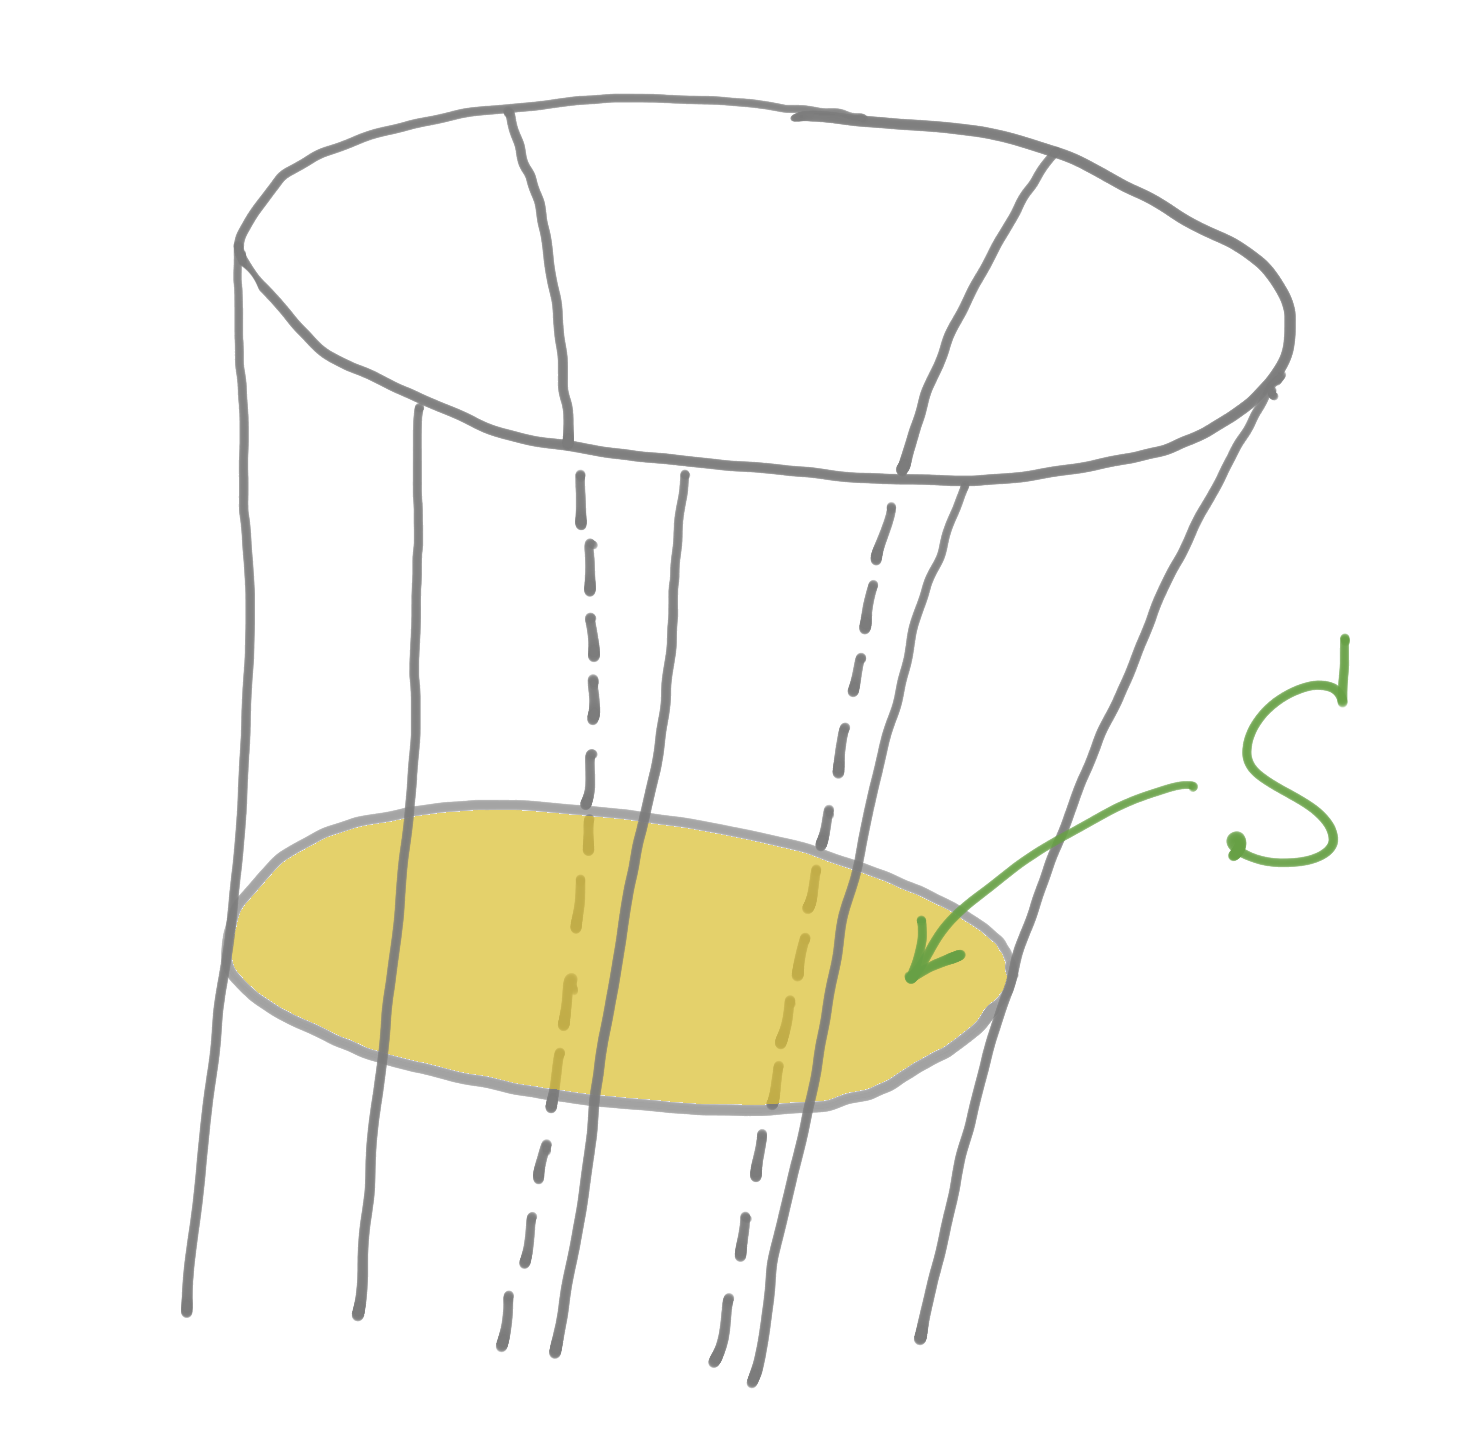
\includegraphics[width=0.5\linewidth]{pics/ch10.5.png}
    \caption{\label{fig:ch10.5}
    {\color{red} Вихревая трубка. \textbf{ОПИСАТЬ!!! }}
    }
    \end{figure}    
Как только мы определим вихревую трубку мы можем сравнить силу или интенсивность одной вихревой трубки с другой. Мы можем сделать это определить число (скаляр)
\begin{equation}
    \label{eq:ch10-gamma}
    \Gamma=\int_S\vec{\zeta}\cdot\vec{\eta} d\sigma=\int_S \vec{\eta}\cdot(\nabla\times V)d\sigma
\end{equation}
здесь $\vec{\zeta}$ -- вектор вихря, а $\vec{\eta}$ -- единичная нормаль к поверхности $S$. Эта величина называется циркуляцией. Она называется так потому, что по теореме Стокса имеет место соотношение
\begin{equation}
    \label{eq:ch10-stoks}
    \iint_S \vec{\eta}\cdot(\nabla\times\vec{B})d\sigma = \int_C\vec{\tau}\cdot \vec{B} dS,
\end{equation}
где $\vec{B}$ -- вектор, имеющий непрерывные первые производные и определенный на поверхности $S$, $\vec{\eta}$ -- нормаль по отношению к $S$, $\vec{\tau}$ -- вектор, тангенциальный к кривой $C$, ограничивающий $S$.

\begin{info}
    Это соотношение было на самом деле получено впервые Кельвином при изучении им вихря, но в литературе почти всюду приписывается Стоксу, который использовал его в своей работе в 1854, ознакомившись с ним до этого из письма Кельвина, адресованного ему.
\end{info}

С использованием теоремы Стокса (\ref{eq:ch10-gamma}) может быть представлено в виде
\begin{equation}
    \label{eq:ch10-gamma1}
    \Gamma = \int_C \vec{\tau}\cdot\vec{V}dS
\end{equation}
Таким образом циркуляция есть сумма компонентов скорости, тангенциальной к кривой $C$.

\section{{\color{done}Уравнение спиральности}}
ПОмимо более традиционных характеристик потоков, таких как завихренность, потенциальная завихренность, энергия, в последние годы в метеорологии приобретает определенную популярность концепция спиральности течений. 

Понятие спиральности было введено в гидромеханике в начале 60-х годов 20 прошлого столетия. Спиральность определяется как скалярное произведение вектора скорости, на вектор вихря
\begin{equation}
    \label{eq:ch10-curt}
    h = \nabla\times\vec{V}\cdot\vec{V}
\end{equation}
Удобной характеристикой поля спиральности является относительная спиральность
\begin{equation}
    \label{eq:ch10-relcurt}
    rh= (\nabla\times\vec{V}\cdot\vec{V})/( |\nabla\times\vec{V}| \cdot |\vec{V}| )= cos{ ( \widehat{ \nabla\times\vec{V}\cdot\vec{V} } ) }
\end{equation}
представляя собой косинус угла между векторами скорости и завихренности, что следует из скалярного произведения векторов.
\begin{info}
    \begin{equation*}
        \vec{a} \cdot \vec{b} = a \cdot b \cos{\theta}; \:\: \cos{\theta} = \frac{\vec{a} \cdot \vec{b}}{a \cdot b}.
    \end{equation*}
\end{info}
Относительная спиральность изменяеться в пределах $-1\leq rh \leq 1$. Теоретически максимальное значение $| rh | = 1$ достигается в тау называемых винтовых течениях, где $\nabla\times\vec{V}\cdot\vec{V}=0$ или в случае атмосферы $\vec{\omega_a}\times\vec{V}=0$, где $\vec{\omega_a}$ -- абсолютный вихрь. Из определения $rh$ (\ref{eq:ch10-relcurt}) видно, что при винтовых течениях векторы ветра и завихренности являеются колинеарными, поэтому взаимодействие их перекрестных проихводных типа $\omega_x u_y - \omega_y u_x$ (пример для вертикальной оси) исчезает. Это приводит к тому, что системы течений с большой спиральностью б\textit{о}льшим временем жизни, чем системы с малой спиральностью, как характеристика состояния потока в некоторой области, и представляет определенный интерес. Отметим дополнительно, что в установившихся винтовых течениях при отсутствии притоков тепла потенциальный вихрь Эртеля
\begin{equation*}
    q=\frac{\vec{\omega}\cdot\nabla\sigma}{\rho} = 0,
\end{equation*}
где $\sigma$ -- удельная энтропия. В реальной вязкой атмосфере с притоками и стоками тепла винтового движения в $rh=1$, естественно, не достигается, но тенденции к увеличению спиральности в отдельных районах атмосферы могут иметь место и служить признаком того, что циркуляция в этом районе более устойчива, а потому более прогнозируемой.

Ниже будет выведено уравнение спиральности, описывающие индивидуальное изменение спиральности в движущейся частице. 

Компоненты спиральности по осям $x$, $y$,$z$ будем обозначать $h_x$,$h_y$,$h_z$. Уравнение спиральности образуется из уравнению движения и уравнения вихря, которые мы напишем покомпонентно для случая идеальной жидкости
\begin{align}
    \omega_x \times &\bigg| \:\: \td{u}{t} = -\alpha\pd{p}{x}+fv \label{eq:ch10-curl-dudt} \\  
    \omega_y \times &\bigg| \:\: \td{v}{t} = -\alpha\pd{p}{y}-fu \label{eq:ch10-curl-dvdt} \\ 
    \omega_z \times &\bigg| \:\: \td{w}{t} = -\alpha\pd{p}{z}+g  \label{eq:ch10-curl-dwdt} \\ 
    u \times &\bigg| \:\: \td{\omega_x}{t} = 
            \omega_x\pd{u}{x} + \omega_y\pd{u}{y} + \omega_z\pd{u}{z} + f\pd{u}{z} - 
            \omega_x \nabla\cdot\vec{U} -\rb{ \pd{\alpha}{y}\pd{p}{z} - 
            \pd{\alpha}{z}\pd{p}{y} } \label{eq:ch10-omegax} \\ 
    v \times &\bigg| \:\: \td{\omega_y}{t} = 
            \omega_x\pd{v}{x} + \omega_y\pd{v}{y} + \omega_z\pd{v}{z} + f\pd{v}{z} - 
            \omega_y \nabla\cdot\vec{U} -\rb{ \pd{\alpha}{z}\pd{p}{x} - 
            \pd{\alpha}{x}\pd{p}{z} } \label{eq:ch10-omegay} \\ 
    w \times &\bigg| \:\: \td{\omega_z}{t} = 
            \omega_x\pd{v}{x} + \omega_y\pd{v}{y} + \omega_z\pd{v}{z} - \beta v  - 
            (f+\omega_z) - \rb{ \pd{\alpha}{x}\pd{p}{y} - 
            \pd{\alpha}{y}\pd{p}{x} } \label{eq:ch10-omegaz} 
\end{align}
Состояние спиральности по разным осям определяются домножением уравнений (\ref{eq:ch10-curl-dudt})-(\ref{eq:ch10-curl-dwdt}) на соответствующие компоненты вихря: $\omega_x$, $\omega_y$ и $\omega_z$, а уравнений для различных компонентов вихря (\ref{eq:ch10-omegax})-(\ref{eq:ch10-omegaz}) на соответствующие компоненты вектора скорости: $u$, $v$ и $w$. Напишем подробно образование уравнения для вертикального компонента спиральности $h_z$, а остальные выпишем уже в готовом виде. Итак, умножая уравнение (\ref{eq:ch10-curl-dwdt}) на $\omega_z$, а уравнение (\ref{eq:ch10-omegaz}) на $w$, будем иметь
\begin{align*}
    \td{h_z}{t} = w\omega_x\pd{w}{x} + w\omega_y\pd{w}{y} + w\omega_z\pd{w}{z} + 
      - w(\nabla\cdot\vec{U}(f+\omega_z)) - w\beta v - \\
      - w \rb{ \pd{\alpha}{x}\pd{p}{y} - \pd{\alpha}{y}\pd{p}{x} } - \omega_z \rb{ \alpha\pd{p}{z}+g }
\end{align*}
Можно сгруппировать члены этого уравнения в том же порядке, как это делалось для уравнения вихря
\begin{multline}
    \td{h_z}{t} = \frac{1}{2} \ub{ \qb{ \omega_x\pd{w^2}{x} + \omega_y\pd{w^2}{y} + \omega_z\pd{w^2}{z} } }_{1} - 
    \ob{\tikzmark{ch10-4}w(f+\tikzmark{ch10-5}\omega_z)(\nabla\cdot\vec{U}) - w\beta v }^{2} - \\
  - \ub{ w \rb{ \pd{\alpha}{x}\pd{p}{y} - \pd{\alpha}{y}\pd{p}{x} } }_{3} - 
    \ub{ \omega_z \rb{ \alpha\pd{p}{z}+g } }_{4} \label{eq:ch10-curl1}
\end{multline}
    \begin{tikzpicture}[remember picture,overlay]
        \draw[<->]
        ([shift={(2pt,-2pt)}]ch10-4)
        -- ([shift={(2pt,-12pt)}]ch10-4)
        -- node[midway, below] {$\scriptstyle h_z$} ([shift={(2pt,-12pt)}]ch10-5)
        -- ([shift={(2pt,-2pt)}]ch10-5);
    \end{tikzpicture}
Сравнивая это уравнение с уравнением для вертикального компонента завихренности, можно увидеть, что они в значительной мере схожи друг с другом. В правой части первые три члена определяют генерацию спиральности. Если иметь ввиду для определенности положительную спиральность, то можно заметить, что она будет генерироваться горизонтальной завихренностью в тех местах, где $\pd{w^2}{x}>0$ и $\pd{w^2}{y}>0$, то есть там где $w$ и горизонтальные градиенты $w$ имеют один и тот же знак. Третье слагаемое усиливает уже имеющуюся положительную спиральность в области, где совпадают знаки $w$ и $\pd{w^2}{x}$. Четвертое слагаемое указывает на то, что в области восходящих течений наличие конвергенции увеличивает уже существующую спиральность. Здесь же следует отметить, что в области восходящих потоков и конвергенции спиральность всегда увеличивается под действием вращения Земли, т.к. $\beta=\pd{f}{y}>0$, то в области $w>0$ положительная спиральность генерируется при $v<0$. Действие соленоидальных членов будет генерировать спиральность при отрицательных значениях множителя стоящего в круглых скобках. По сравнению с уравнением вихря в уравнении спиральности появляется дополнительная группа членов (два последних слагаемых в уравнении). При реальном распределении давления по вертикали $\pd{p}{z}<0$ первое слагаемое при $\omega_z > 0$ всегда генерирует положительную спиральность, а второй член всегда ее уменьшает.

В частном случае несжимаемой жидкости $ \rb{ \alpha=\frac{1}{\rho}=0 }$ уравнение для вертикального компонента спиральности приобретает вид
\begin{equation}
    \label{eq:ch10-curl2}
    \td{h_z}{t} = \frac{1}{2} \qb{ \omega_x\pd{w^2}{x} +\omega_y\pd{w^2}{y} +\omega_z\pd{w^2}{z} } - w\beta v - \omega_z \rb{ \alpha\pd{p}{z} + g }
\end{equation}
Члены с $\nabla\cdot\vec{U}$ и $\pd{\alpha}{x}$, $\pd{\alpha}{y}$ (соленоидальный член) из этого уравнения исчезли. На малых масштабах течений при сохранении условий несжимаемости можно исключить член с $\beta$-эффектом, на больших масштабах можно исключить член с наклоном горизонтальной завихренности.

Уравнения для спиральности по осям $Ox$ и $Oy$ имеют следующий вид
\begin{align}
    \td{h_x}{t} = \frac{1}{2} \qb{ \omega_x\pd{u^2}{x} + \omega_y\pd{u^2}{y} + (\omega_z+f)\pd{u^2}{z} } - h_x (\nabla\cdot\vec{U}) - \\
    - u \rb{ \pd{\alpha}{y}\pd{p}{z} - \pd{\alpha}{z}\pd{p}{y}  } - \omega_x \rb{ \alpha\pd{p}{x}+fv } \label{eq:ch10-curlx} \\
    \td{h_y}{t} = \frac{1}{2} \qb{ \omega_x\pd{v^2}{x} + \omega_y\pd{v^2}{y} + (\omega_z+f)\pd{v^2}{z} } - h_y (\nabla\cdot\vec{U}) - \\
    - v \rb{ \pd{\alpha}{z}\pd{p}{x} - \pd{\alpha}{x}\pd{p}{z}  } - \omega_y \rb{ \alpha\pd{p}{y}+fu } \label{eq:ch10-curly} 
\end{align}
Все члены, которые не содержат силы Кориолиса, легко представляются с помощью единого уравнения по повторяющимся индексам. Члены, содержащие параметр Кориолиса, были значительно упрощены с самого начала, в них отсутствует симметрия в кравнениях движения, поэтому оставляем их в явном и громоздком виде. Итак, по повторяющимся индексам $i=1,2,3; \:\: j=1,2,3$ уравнение спиральности можно представить в виде 
\begin{equation}
    \label{eq:ch10-curl_ij}
    \td{h_i}{t} = \frac{1}{2} \omega_{ai}\pd{u_{i}^2}{x_j} - 
        h_{ai} (\nabla\cdot\vec{U}) - 
        \omega_i\alpha\pd{p}{x_i} - 
        u_i \rb{ \nabla\alpha\times \nabla p }_i - 
        \ub{u_3 u_2}_{wv} \beta + 
        f (\ub{\Omega_1 u_2 - \omega_2 u_1}_{2(\vec{\omega}\times\vec{V})_{i=3}})
\end{equation}
Здесь под $h_{ai}$ понимается $h_{ai}=(h_i+f)$, $f\neq0$ при $i=3$ т.к. мы используем в наших уравнениях только вертикальный компонент завихренности Земли, то $f_1, f_2=0, f_3\neq0$. 

\begin{warn}
    На будущее: нужно сравнить с уравнением завихренности и написать в векторной форме $\td{(\vec{\omega}\cdot\vec{V})}{t}=...$
\end{warn}

\section{{\color{done}Уравнение энергии}}
Энергией называется всякая физическая величина, имеющая размерность $ML^2/T^2$, например $ \textrm{кг} \cdot \textrm{м}^2 / \textrm{с}^2= \textrm{Дж}$. Понятие энергии, таким образом, дает общую меру для качественно различных видов движения материи. В изолированной системе могут происходить превращения энергии одного вида в энергию другого вида, но общее количество энергии (полная энергий) остается неизменным.

Прежде всего дадим определение наиболее важных видов энергии.
\begin{enumerate}
  \item Гравитационная потенциальная энергий некоторого элемента воздушного столба есть
    \begin{equation*}
        dE_p = g z dm = gz \ub{\rho(x,y,z)dxdydz}_{dm}, 
          \:\: \qb{ \frac{\scriptstyle \textrm{кг} \: \textrm{м} }{\scriptstyle \textrm{с}^2} }
    \end{equation*}
    Потенциальная энергия, отнесенная к единице массы есть
    \begin{equation*}
        E_p = g z \:\: \qb{ \frac{\scriptstyle \textrm{м}^2 }{\scriptstyle \textrm{с}^2} }
    \end{equation*}
    При рассмотрении энергетики атмосферы могут использоваться как первое, так и второе определение энергии. Потенциальная энергий характеризует потенциал, который приобретает тело, в т.ч. и частица воздуха, будучи поднятой на высоту $z$ в поле тяготения $g$.
    \item Внутренняя энергия некоторого элемента воздушного столба есть
    \begin{equation*}
        E_p = C_v T \ub{\rho(x,y,z)dxdydz}_{dm}, \:\: \qb{ \frac{\scriptstyle \textrm{кг} \: \textrm{м}}{\scriptstyle \textrm{с}^2} }, \:\: C_v = \qb{ \frac{\scriptstyle \textrm{м}^2}{\scriptstyle (\textrm{с}^2 \:\: \textrm{град} } }
    \end{equation*}
    Внутренняя энергия, отнесенная к единице массы, есть
    \begin{equation*}
        dE_{in} = C_v T, \:\: \qb{  \frac{\scriptstyle \textrm{м}^2 }{\scriptstyle \textrm{с}^2} }
    \end{equation*}
    \item Кинетическая энергий 
    \begin{equation*}
        E_k = \frac{V^2}{2}\rho dxdydz \:\: 
        \qb{ \textrm{кг} \frac{\scriptstyle \textrm{м}^2 }{\scriptstyle \textrm{с}^2} }, \:\:
        \textrm{где} \:\: V^2=u^2+v^2+w^2
    \end{equation*}
    Отнесенная к единице массы кинетическая энергия есть
    \begin{equation*}
        E_k = \frac{V^2}{2} \:\: 
        \qb{ \frac{\scriptstyle \textrm{м}^2 }{\scriptstyle \textrm{с}^2} }
    \end{equation*}
\end{enumerate}
    
\begin{warn}
    Пропущен блок со пояснениями $\vec{V} \cdot (-2\vec{\Omega \times \vec{V}})=0$. Непонятно зачем это вообще нужно. 
\end{warn}

\subsection{{\color{done}Вывод уравнения энергии}}
Уравнение энергии связывает различные виды энергии, которыми обладает движущаяся атмосфера. 

Для образования уравнения полной энергии нам понадобятся уравнения движения, характеризующие кинематическую энергию и потенциальную энергию частицы, находящейся в поле силы тяжести.

Выпишем векторную форму уравнений движения
\begin{equation}
    \label{eq:ch10-ee-1}
    \td{\vec{V}}{t} = -\alpha\nabla p - 2 (\vec{\Omega} \times \vec{V})+\vec{g}+\vec{F}, \:\: \textrm{где} \:\: \alpha=\frac{1}{\rho}
\end{equation}
Так как сила тяжести действует только вдоль оси $z$, будем использовать далее ее скалярное значение. Умножим скалярно уравнение (\ref{eq:ch10-ee-1}) на вектор скорости $\vec{V}$ и получим следующее уравнение
\begin{equation}
    \label{eq:ch10-ee-2}
    \td{\vec{V} \cdot \vec{V}}{t} = -\alpha\vec{V} \cdot \nabla p - 2 (\vec{\Omega} \times \vec{V})-wg+\vec{V} \cdot \vec{F}.
\end{equation}
Некоторая гибридная запись уравнения (\ref{eq:ch10-ee-2}) связана с тем, что образование уравнения (\ref{eq:ch10-ee-2}) из уравнение (\ref{eq:ch10-ee-1}) происходит почленным умножением компонентов вектора $\vec{V}$ на уравнения движения для тех же самых компонентов. Поэтому в уравнении для $w$ в правой части и появляется член $-wg$, содержащий только вертикальный компонент скорости. Далее, член с силой Кориолиса пропадает, т.к. $\vec{V} \cdot (-2\vec{\Omega \times \vec{V}})=0$. Таким образом \underline{сила Кориолиса работы не производит}, она действует только отклоняющим образом на движения, возникающие во вращающейся среде. Остальные члены в правой части интерпретируются следующим образом. $-\alpha (\vec{V} \cdot \nabla p)$ -- работа, затраченная на силой градиента давления в единице массы воздуха за единицу времени. $\vec{V} \cdot \vec{F}$ -- работа, затраченная силой трения в единице массы воздуха за единицу времени. Так как $\vec{V} \cdot \vec{V} = V^2 = (u^2+v^2+w^2)$ и $w=\td{z}{t}$, а $g=const$, то уравнение (\ref{eq:ch10-ee-2}) можно переписать в виде
\begin{equation}
    \label{eq:ch10-ee-3}
    \td{}{t} \rb{ \frac{V^2}{2} + gz } = -\alpha\vec{V} \cdot \nabla p +\vec{V} \cdot \vec{F}, 
\end{equation}
где $\frac{V^2}{2}$ -- кинетическая энергия в единице массы, $gz$ -- потенциальная энергия в единице массы в поле тяготения. 

Первый закон термодинамики есть 
\begin{equation}
    \label{eq:ch10-ee-4}
    dQ = dE + pd\alpha.
\end{equation}
Он обозначает, что количество тепла, сообщенное единице массы равно изменению внутренней энергии на единицу массы и работе за счет расширения невязкого газа (это частный случай, т.к. работа, произведенная единицей массы данной системы $dW$ сводится лишь к работе за счет расширения газа).

Далее из термодинамики нам известно, что приращение внутренней энергии может быть представлено в виде
\begin{equation*}
    dE = C_v dT.
\end{equation*}
И уравнение (\ref{eq:ch10-ee-4}) можно переписать таким образом в виде
\begin{equation*}
    dQ = C_v dT + pd\alpha.
\end{equation*}
Переходя в измерению (притоку) тепла в частице, получи
\begin{equation}
    \label{eq:ch10-ee-5}
    \td{Q}{t} = C_v td{T}{t} + p \td{d\alpha}{t}.
\end{equation}
Теперь поменяем знак в уравнении (\ref{eq:ch10-ee-5}) на обратный и сложим с уравнением (\ref{eq:ch10-ee-3}). Получим
\begin{equation}
    \label{eq:ch10-ee-6}
    \td{}{t} \rb{ \frac{V^2}{2} + gz + C_v T} = \td{Q}{t} - p \td{\alpha}{t} - \alpha\vec{V} \cdot \nabla p +\vec{V} \cdot \vec{F}.
\end{equation}
Выпишем теперь уравнение для индивидуальной производной давления
\begin{equation*}
    \td{p}{t} = \pd{p}{t}+\vec{V} \cdot \nabla p  \:\: \textrm{или} \:\: 0=-\td{p}{t} + \pd{p}{t}+\vec{V} \cdot \nabla p
\end{equation*}
Добавим его к уравнению (\ref{eq:ch10-ee-6}), умножив его предварительно на $\alpha$, получим
\begin{equation*}
    \label{eq:ch10-ee-7}
    \td{}{t} \rb{ \frac{V^2}{2} + gz + C_v T} = 
    \td{Q}{t} - \alpha\td{p}{t} + \alpha\pd{\tikzmark{ch10_41}p}{t} + \cancel{\alpha\vec{V} \cdot \nabla p} - p\td{\tikzmark{ch10_42}\alpha}{t} - \cancel{\alpha\vec{V} \cdot \nabla p} + \vec{V} \cdot \vec{F}
\end{equation*}
    \begin{tikzpicture}[remember picture,overlay]
        \draw[<->]
        ([shift={(2pt,-20pt)}]ch10_41)
        -- ([shift={(2pt,-25pt)}]ch10_41)
        -- node[midway, below] {$ \scriptstyle -\frac{d(\alpha p)}{dt} $} ([shift={(2pt,-25pt)}]ch10_42)
        -- ([shift={(2pt,-20pt)}]ch10_42);
    \end{tikzpicture}
    или
\begin{equation}
    \label{eq:ch10-ee-7}
    \td{}{t} \rb{ \frac{V^2}{2} + gz + C_v T} = 
    \td{Q}{t} + \alpha\pd{p}{t} + \vec{V} \cdot \vec{F}.
\end{equation}
Рассмотрим теперь два последних слагаемых в левой части уравнения. Из уравнения состояния имеем $p\alpha = RT$, кроме того $C_p=C_v+R$, откуда $C_v=C_p-R$. Подставляя эти соотношения в (\ref{eq:ch10-ee-7}), получим
\begin{equation*}
    (C_p-R)T+RT = C_pT-\cancel{RT}+\cancel{RT}
\end{equation*}
или 
\begin{equation}
    \label{eq:ch10-ee-8}
    \td{}{t} \rb{ \frac{V^2}{2} + \ub{C_pT}_{\textrm{энтальпия}} + gz } = \td{Q}{t} + \alpha\pd{p}{t}+\vec{V} \cdot \vec{F}.
\end{equation}
В левой части (\ref{eq:ch10-ee-8}) имеем таким образом полную энергию частицы (кинетическую + внутреннюю + потенциальную), а в правой части источники и стоки полной энергии.

Если движения являются адиабатическими $ \rb{\td{Q}{t}=0} $, отсутствует трение $(\vec{F}=0)$ и течение установившееся $ \rb{ \pd{p}{t} = 0 } $, то полная энергия в частице будет сохраняться
\begin{equation}
    \label{eq:ch10-ee-9}
    \td{}{t} \rb{ \frac{V^2}{2} + C_pT + gz } = 0.
\end{equation}
Можно сформулировать это более аккуратно: в установившемся адиабатическом движении без трения сумма кинематической, потенциальной и энергии и энтальпии (внутренней энергии) сохраняется (остается постоянной).

\subsubsection{{\color{done}Переходы энергии}}
На основе выведенных выше уравнений можно произвести анализ переходов одной формы энергии в другую.

\textbf{Переход от потенциальной энергии в кинетическую}. Для перехода нам достаточно воспользоваться (\ref{eq:ch10-ee-9}) и исключить из рассмотрения энтальпию. Будем иметь из (\ref{eq:ch10-ee-9})
\begin{equation*}
    \td{}{t} \rb{ \frac{v^2}{2}} = -d\td{z}{t}=-gw
\end{equation*}
или
\begin{equation*}
    C(E_P,E_K)=-gw, 
\end{equation*}
где $E_P$ -- потенциальная энергий, а $E_K$ -- кинетическая. Т.е. если скорость направлена вдоль силы тяжести ($w<0$), то кинетическая энергий растет, если против силы тяжести то убывает.

\textbf{Переход внутренней энергии в кинетическую}. В этом случае исключим из рассмотрения потенциальную энергию и силы трения, т.к. они в данном случае роли не играют. Из первого начала термодинамики (\ref{eq:ch10-ee-4}) будем иметь 
\begin{equation}
    \label{eq:ch10-ee-10}
    \td{Q}{t}=\td{E}{t}+p\td{\alpha}{t},
\end{equation}
а уравнение энергии (\ref{eq:ch10-ee-6}) для рассматриваемого частного случая примет вид
\begin{equation*}
    \td{}{t} \rb{ \frac{V^2}{2} } + \td{E}{t}= \td{Q}{t} - p \td{\alpha}{t} - \alpha\vec{V} \cdot \nabla p.
\end{equation*}
Заменяя в последнем выражении $\td{Q}{t}$ из (\ref{eq:ch10-ee-10}) получим
\begin{equation}
\label{eq:ch10-ee-11}
    \td{}{t} \rb{ \frac{V^2}{2} } = - \alpha\vec{V} \cdot \nabla p.
\end{equation}
Поэтому переход внутренней энергии в кинетическую есть 
\begin{equation}
\label{eq:ch10-ee-12}
    C(E_E,E_K) = - \alpha\vec{V} \cdot \nabla p.
\end{equation}
Очевидно, что $C(E_K,E_E) = -C(E_E,E_K)$.

\textbf{Переход внутренней и потенциальной энергии в кинетическую}. 
\begin{equation*}
    C(E_E+E_P,E_K) = - (\alpha\vec{V} \cdot \nabla p + wg)
\end{equation*}
или в более общем случае 
\begin{equation}
    \label{eq:ch10-ee-13}
    C(E_E+E_P,E_K) = -\vec{V}(\alpha\nabla p + g\vec{k}).
\end{equation}
Можно показать, что член с трением в уравнениях (\ref{eq:ch10-ee-3}) и (\ref{eq:ch10-ee-6}) всегда отрицателен. Мы этого доказывать не будем, а примем к сведению. В этом случае из (\ref{eq:ch10-ee-13}) следует, что для поддержания или повышения кинетической энергии системы необходимо, чтобы выполнялось условие
\begin{equation*}
    C(E_E+E_P,E_K) > 0.
\end{equation*}
Рассмотрим теперь \textbf{влияние отдельных членов}. Член с давлением если написать покомпонентно, будет давать (см \ref{eq:ch10-ee-2})
\begin{equation*}
    \td{}{t} E_{K_i} = - \int_{V_M}v_i\pd{p}{x_i}dV_M = \int_{V_M}p\pd{v_i}{x_i}dV_M=\int_{V_M}p(\nabla\cdot\vec{V})dV_M,
\end{equation*}
где $V_M$ -- материальный объем, т.е. объем, сохраняющий из одних и тех же частиц воздуха и движущийся вместе с потоком, будем иметь $\td{}{t}E_{K_1}+\td{}{t}E_{K_2}+\td{}{t}E_{K_3}=0$, т.к. $\nabla\cdot\vec{V}=0$. Т.е. градиент давления переносит энергию одного компонента скорости к другому. В сжимаемой жидкости градиент давления переводит часть энергии также во внутреннюю из кинетической или наоборот, но в атмосферных условиях член $\td{p}{t}$ невелик по сравнению с $\rho (\nabla\cdot\vec{V})$, поэтому и в сжимаемой жидкости градиент давления в основном перераспределяет энергию между компонентами вектора скорости.

Гравитационный член
\begin{equation*}
    \td{}{t}E_{K_3} = -\int_V g\rho w dV
\end{equation*}
переносит энергию от потенциальной к кинетической или наоборот. Нетрудно заметить, что все зависит от комбинации плотности и вертикальной скорости. Если представим плотность в виде пульсирующего от некоторого стандартного значения $\rho_0$, то это будет обозначать что при $\rho^{'}<0$ и $w>0$ кинетическая энергия растет т.е. менее плотный воздух в поле восходящих потоков дает увеличение $E_K$. Аналогично кинетическая энергия растет при $\rho^{'}>0$ и $w<0$, т.е. более плотный воздух в поле нисходящих течений ускоряется и дает рост $E_K$. В гидростатической атмосфере вертикальный компонент кинетической энергии черпается только из горизонтальных компонентов кинетической энергии или внутренней энергии посредством вертикального градиента давления.


Член с ускорением Кориолиса, как мы уже говорили, не является источником или стоком энергии, а только переводит энергию от одного компонента скорости к другому.

Мы использовали до сих пор индивидуальную производную, т.е. исследовали изменение энергии в движущейся частице. Если бы мы рассмотрели изменение кинетической энергии в точке, то появилась бы группа инерционных нелинейных членов. Мы не будем подробно доказывать вывод, который можно получить. Он состоит в том, что вклад инерционного члена для каждого компонента равен нулю, т.е. эффект этого члена состоит только в перераспределении энергии внутри потока, что создаст бесконечно множество систем течений. 



\section{Уравнение дивергенции скорости}

\section{Уравнение тенденции}

